\documentclass[a4paper,12pt,oneside,chapterprefix=true]{scrbook}
\usepackage[utf8]{inputenc}
\usepackage[T1]{fontenc}
\usepackage[top=2.5cm, bottom=2.5cm, left=2.5cm, right=2.5cm]{geometry}
\usepackage[osf,sc]{mathpazo}
\usepackage[citecolor=magenta,colorlinks=true,hypertexnames=false,pdftitle=Mémoire SERENA Gbodjo]{hyperref}
\usepackage{natbib}
\usepackage[english,french]{babel}
%\usepackage{setspace}
%\usepackage{makeidx}
%\usepackage[french]{nomencl}
\usepackage[acronyms,xindy,toc,nomain]{glossaries}
\usepackage{graphicx}
\usepackage{cleveref}
\usepackage{amsmath,amssymb,mathrsfs}
\usepackage{tikz}
\usepackage{pgfplots}\usepgfplotslibrary{dateplot}\usetikzlibrary{shapes,arrows}
\usepackage{pdfpages}
\usepackage{textcomp}
%\usepackage{shorttoc}
\usepackage{siunitx}
%\usepackage{fancyhdr}

%\title{Evaluation du potentiel d’une série temporelle multi-source à haute résolution spatiale pour le suivi des cultures annuelles en petite agriculture familiale : 
%Cas du bassin arachidier sénégalais}
%\author{\textsc{Gbodjo} Yawogan Jean Eudes}
%\date{\today}

%\onehalfspacing
\pagestyle{plain}
%\renewcommand{\emph}{\textbf}

\makeglossaries
\pgfplotsset{compat=1.15}

\newenvironment{abstract}%
{\cleardoublepage\thispagestyle{empty}\null\vfill\begin{center}%
\sffamily\bfseries \abstractname \end{center}}%
{\vfill\null}

\newenvironment{acknowledgements}%
{\cleardoublepage\thispagestyle{empty}\null\vfill\begin{center}%
\sffamily\bfseries Remerciements \end{center}}%
{\vfill\null}

\addto\captionsfrench{\renewcommand{\contentsname}{Sommaire}}

\begin{document}
\let\cleardoublepage\clearpage

\includepdf[pages=1]{Garde.pdf}
%\maketitle

\frontmatter
  
  \setcounter{tocdepth}{2}
  \selectlanguage {french}
    \begin{abstract}

    \end {abstract}
    
  \selectlanguage {english}
    \begin {abstract}

    \end{abstract}

  \selectlanguage {french}
  
    \begin{acknowledgements}

    \end{acknowledgements}

  %\shorttoc{Sommaire}{2}
  \tableofcontents
  \listoffigures
  \listoftables
  

\mainmatter

  \chapter{Introduction}
  
  %\newacronym{cirad}{CIRAD}{Centre de Coopération Internationale pour la Recherche Agronomique et le Développement} 
%\newacronym{aida}{Aïda}{Agroécologie et intensification durable des cultures annuelles}
%\newacronym{isra}{ISRA}{Institut Sénégalais de Recherche Agronomique}
%\newacronym{cse}{CSE}{Centre de Suivi Ecologique}

\section{Introduction}

La \emph{sécurité alimentaire} désigne \og une situation garantissant à tout moment, à tous les êtres humains, la possibilité physique, sociale et économique 
de se procurer une nourriture suffisante, saine et nutritive leur permettant de satisfaire leurs besoins et préférences alimentaires pour mener une vie saine et active \fg{}
tel que défini par le Comité de la Sécurité alimentaire mondiale. On considère généralement \emph {quatre piliers} ou dimensions de la sécurité alimentaire : l'Accès (la plus mise 
en avant), la Disponibilité, la Qualité et la Stabilité. Aujourd'hui la notion d'Excès est également évoquée quand l'on sait qu'un régime alimentaire malsain peut être à la cause 
de l'obésité, du surpoids ou de maladies comme l'hypertension artérielle. Selon la FAO (Rapport SOFI 2017), 815 millions de personnes en 2016, soit plus d'une personne sur dix, 
seraient en situation d'insécurité alimentaire. Les facteurs de l'insécurité alimentaire sont divers. La pénurie d'eau, la dégradation des sols, le changement climatique, les épidémies, 
l'explosion démographique ou encore les situations de conflits sont autant de sources antérieures à une telle situation. \\L'un des défis majeurs de notre temps est de garantir à une 
population toujours plus grandissante (près de 10 milliards en 2050 selon les projections des Nations Unies), une alimentation suffisante pour couvrir ses besoins nutritionnels. 
Ainsi, nourrir 2 milliards de personnes de plus en 2050 nécessitera de revoir à la hausse la production alimentaire mondiale qui devra être globalement augmentée de 50\% (Rapport SOFI 
2017). Face à ce défi, et surtout dans les pays en développement, le concept \og d'\emph{Intensification écologique} ou d'\emph{Agriculture écologiquement intensive} \fg{} trouve 
parfaitement son application. L'intensification écologique est un concept agronomique développé au CIRAD dans le contexte de l'agriculture des pays du Sud, caractérisés par des 
rendements faibles. Il se veut de mettre au point des systèmes de production agricole utilisant de façon intensive, les processus biologiques et écologiques ainsi que leurs 
fonctionnalités naturelles, plutôt que d'utiliser de façon intensive les intrants (énergies fossiles, engrais chimiques, pesticides). L'utilisation intensive de ce facteur de 
production naturel et écosytémique, permettrait ainsi de maintenir des niveaux de rendements élevés, préservant les ressources naturelles et assurant de ce fait une durabilité des
écosystèmes cultivés \cite{Goulet2012}.\\ \`A Niakhar au Sénégal, dans la région du bassin arachidier, l'une des voies de l'intensification écologique repose sur les associations culturales 
entre céréales et légumineuses. Ainsi, l'on retrouve souvent des cultures de \emph{Mil} entresemées de \emph{Niébé} (Haricot) ou d'\emph{Arachide}. Plus encore, l'on note la 
présence d'espèces arborées sur les parcelles cultivées telle que le \emph{Faidherbia Albiba}. Ces différentes pratiques permettraient non seulement d’accroître la fertilité des 
sols et par conséquent la productivité des systèmes de cultures mais aussi de diversifier les sources de revenus et d’alimentation dans les régions rurales où les moyens d’existence
des populations dépendent étroitement des cultures annuelles produites. Par ailleurs, elles permettraient également de limiter l’impact des fluctuations climatiques sur la 
production agricole. Une évaluation spatialisée des rendements des principales cultures alimentaires s'avère donc indispensable pour évaluer les performances agronomiques et 
environnementales des systèmes de cultures. Sur cet aspect, l'intérêt de recourir aux techniques de Télédétection n'est plus à remettre en cause. La Télédétection s'est révelée 
indispensable ces dernières décennies pour le suivi des cultures, la prévision des récoltes ou encore l'estimation de la biomasse et des rendements, sur des échelles régionales et 
globales. De nos jours, la mise au point d'instruments, combinant à la fois haute ou très haute résolution spatiale et haute fréquence temporelle à l'instar de Sentinel-2, ouvre la
voie à des applications de l'ordre de la parcelle. Pour le suivi de l'agriculture en contexte tropical africain, ceci se traduit par l'affranchissement des contraintes liées à 
l'hétérogénéité des pratiques, aux parcellaires de petites tailles ou encore à la présence d’arbre dans les parcelles. 

\section{Contexte du stage}

Le présent stage s'inscrit dans le cadre de recherches portant sur l’évaluation spatialisée des pratiques d’intensification écologique des systèmes de cultures à base de Mil au 
Sénégal, dans la région du bassin arachidier par Télédétection. Ces travaux sont conduits par le CSE et l'ISRA (Dakar, Sénégal) et l'unité de recherche (UR) A\"ida (CIRAD --- 
Montpellier, France) et sont relatifs aux projets GloFoodS SERENA, SIMCo et LYSA. 

  \subsection{Présentation des Organismes d'accueil}
  
  \begin{itemize}
   \item[.] CSE 
   \item[.] ISRA
   \item[.] UR Aïda --- CIRAD
  \end{itemize}

  
    \paragraph{CSE :}
    
    Le CSE
    
    \paragraph{ISRA :}
    
    L'ISRA 
    
    \paragraph{UR Aïda --- CIRAD :}
    
    L'unité de recherche Aïda du CIRAD 
  
  \subsection{Projets GloFoodS SERENA, SIMCo et LYSA}

\section{Objectifs et Hypothèses}

L'objectif de ce stage est de mener une première analyse des potentialités offertes par une série temporelle multisource à haute résolution spatiale pour le suivi des systèmes 
de cultures à base de Mil, à Niakhar dans le bassin arachidier sénégalais. De manière plus concrète, il s'agira :
\begin{itemize}
   \item d'évaluer et cartographier les dates de semi des différentes parcelles
   \item et de calibrer un modèle statistique d'estimation des rendements.
  \end{itemize}
Pour ce faire, nous travaillerons avec une série temporelle composée d'images \emph{PlanetScope}, \emph{RapidEye} et \emph{Sentinel-2}. Nous disposons également de données de terrain décrivant les 
parcelles notamment leurs caractéristiques et caractéristiques .
Ce travail vient à l'amont d'une étude plus complète visant à évaluer à l’échelle d’un paysage, l’impact de la biodiversité paysagère sur la productivité des systèmes de cultures 
et les potentiels d’intensification des pratiques.

\section{Planning de travail}

Ces tâches ont été réparties dans le temps selon le diagramme de Gantt présenté dans l'annexe A.
  
  \chapter{Contexte et Objectifs}
  
  \section{Contexte du stage}

Le présent stage s'inscrit dans le cadre de recherches portant sur l’évaluation spatialisée par télédétection des pratiques d’intensification écologique des systèmes de cultures à base de mil et d’arachide au Sénégal, dans la région du bassin arachidier. Ces travaux sont relatifs aux projets GloFoodS SERENA, SIIL SIMCo et TOSCA LYSA et sont conduits par 
l'\acrshort{aida} (Cirad --- Montpellier, France) conjointement avec ses partenaires sénégalais le \acrshort{cse} et l'\acrshort{isra} (Dakar, Sénégal).

  \subsection{Présentation des organismes d'accueil}
Ce stage proposé par l’UR Aïda du Cirad s’est déroulé dans les locaux du CSE à Dakar au Sénégal.
    
    \paragraph{L'UR AÏDA}\footnote{\url{https://ur-aida.cirad.fr/}} est une unité de recherche du Cirad créée en 2014 et faisant partie du
département Persyst. Elle se positionne sur l’intensification et la durabilité de la pro-
duction des cultures annuelles en milieu tropical contraint et ses recherches visent la
pleine valorisation des ressources disponibles, en mobilisant les processus écologiques
qui régissent leur dynamique au sein des agrosystèmes. Elle a pour objectif l’étude,
la conception et la proposition de systèmes de culture annuels (canne à sucre, coton-
nier, riz \ldots) répondant aux exigences de performances agronomiques, technologiques
et environnementales. L’unité est structurée en 5 équipes de recherche dont Artists
(Télédétection, systèmes d’information, techniques de simulations et analyses spa-
tiales) pour couvrir les différents aspects de l’intensification écologique et répondre
à la demande sociétale et aux besoins du développement. Ces équipes interagissent
entre elles pour relever ensemble trois grands défis de recherche liés aux systèmes de
culture innovants : la compréhension du fonctionnement de l’agro-écosystème com-
plexe, l’émergence de systèmes de cultures innovants, efficaces et pertinents pour les
agricultures familiales des pays du Sud et l’évaluation de ces systèmes de culture
comme élément essentiel pour la décision et l’action. L’unité dispose d’une large ca-
pacité d’expertise dans les domaines des filières agricoles, de l’environnement, de la
gestion de données ou encore des systèmes d’information et propose des outils, logi-
ciels et analyses à destination des chercheurs et professionnels des filières agricoles.
    
    \paragraph{Le CSE}\footnote{\url{https://www.cse.sn/index.php/fr/}} est un organisme étatique créé en 1986. Il est placé sous la tutelle technique
du ministère en charge de l’environnement et est doté d’une personnalité morale lui
permettant de jouir d’une autonomie administrative et financière. Le CSE a pour mis-
sion de contribuer à la connaissance et à la gestion durable des ressources naturelles et de l’environnement, par la production et la diffusion de produits et services d’aide
à la décision notamment pour l’Etat, les collectivités locales, le secteur privé, la so-
ciété civile, les institutions de recherche et de développement, les organisations de
producteurs et les partenaires au développement. Les domaines d’activités du CSE
couvrent la gestion du littoral, le suivi des zones de parcours, des feux de brousse
et de la production agricole, les études de vulnérabilité et d’adaptation aux change-
ments climatiques, la séquestration de carbone, le suivi à long terme des écosystèmes
ou encore les problématiques d’environnement et santé. Le CSE dispose d’un impor-
tant réseau de partenariat au niveau national (ministères, universités, institutions de
recherches basées à Dakar à l’instar de l’IRD ou du Cirad) comme international (en
Afrique notamment le Centre Agro-hydro-météorologique (AGRHYMET) ou ailleurs
dans le monde comme la FAO ou le PNUE).
    
    \paragraph{L'ISRA}\footnote{\url{https://www.isra.sn}} est un établissement public à caractère scientifique et technologique fondé
en 1974, actuellement sous la tutelle du ministère de l’Agriculture mais disposant de
son propre conseil d’administration. L’ISRA est considéré comme la principale organisation de recherche au Sénégal employant plus de 70\% de chercheurs. L’ISRA a
pour principales missions : la conception et l’exécution de programmes de recherche
sur les productions végétales, forestières, animales et halieutiques et en économie rurale ; la création de connaissances scientifiques, l’innovation technologique et la mise au point d’outils d’aide à la décision pour l’amélioration du secteur agricole ; la valorisation et le transfert des résultats de la recherche ; la promotion et la formation à la recherche par la recherche et le développement de la coopération scientifique aussi
bien interafricaine et internationale qu’avec les institutions de recherche et universités sénégalaises.
    
  
  \subsection{Projets GloFoodS SERENA, SIIL SIMCo et TOSCA LYSA}
  
  \paragraph{SERENA}\footnote{\url{https://www.projects.igeo.fr/projet-1/}} (de la biodiverSité des paysagEs agRicoles à la sEcurité alimeNtAire des
ménages ruraux) est un projet financé dans le cadre du métaprogramme GloFoodS
(Transitions pour la sécurité alimentaire mondiale), un métaprogramme conjoint \acrshort{inra} et Cirad qui a pour objectif de mobiliser les forces scientifiques pluridisciplinaires des deux établissements pour contribuer à éclairer les mécanismes, relevant des écosystèmes et des systèmes socio-économiques, qui sous-tendent les différentes dimensions de la sécurité alimentaire. Le projet SERENA a été proposé par l’UR Aïda et
ses partenaires sénégalais (le CSE, l’ISRA, l’\acrshort{ucad} avec l’objectif d’éclairer la contribution d’un paysage agricole sénégalais diversifié à la sécurité alimentaire et nutritionnelle (SAN) des ménages ruraux. Ce projet est construit autour de l’hypothèse
que la production d’aliments au sein de paysages agricoles polyvalents et diversifiés
peut permettre d’accroître significativement la productivité des systèmes agricoles
et favoriser les sources de revenus et/ou l’accès à des produits diversifiés. Il s’agit
donc de mieux prendre en compte la dimension paysagère dans les études portant
sur la SAN. L’intérêt et l’originalité du projet SERENA est de proposer une démarche
de recherche mobilisant de façon innovante l’écologie du paysage, la télédétection,
la modélisation spatialisée et des enquêtes socio-économiques de ménage pour traiter plusieurs aspects de la SAN à l’échelle d’un paysage sénégalais. Pour ce faire, le projet s’articule autour de 4 axes : l’axe \emph{diversité paysagère} (proposer un plan d’échantillonnage spatialisé à partir d’indicateurs de diversité paysagère et cartographier plus
finement des indicateurs de la biodiversité des paysages agricoles à partir d’images
satellite), l’axe \emph{impact sur les rendements} (analyse du lien entre diversité paysagère et
rendements à l’échelle des parcelles et du paysage), l’axe \emph{SAN et moyens d’existence}
(combiner enquêtes socio-économiques sur les ménages agricoles et indicateurs de
biodiversité paysagère pour renseigner le lien entre diversité paysagère observée et
les stratégies des ménages associées en matière de sécurité alimentaire) et l’axe \emph{Valorisation} (diffusion des résultats du projet auprès de la communauté scientifique et des différents acteurs, à travers un site web intégrant une composante de webmapping et
formations prévues)
  
  
  \paragraph{SIMCo} (Sustainable Intensification of Millet based agrosystems using Cowpea in the Groundnut Basin - Senegal) est un projet financé par le SIIL\footnote{\url{http://www.k-state.edu/siil/index.html}}, laboratoire de l’Univer-
sité du Kansas. Les recherches de ce projet visent une meilleure compréhension des
mécanismes impliqués dans les associations culturales entre mil et niébé et l’estima-
tion de leurs rendements sur divers sites du bassin arachidier sénégalais. De manière
spécifique, les objectifs du projet SIMCo sont : (1) concevoir des agrosystèmes du-
rables à base de céréales et légumineuses en calibrant et en validant des modèles
de cultures associées ; et (2) estimer les rendements des cultures associées au niveau
local et régional. Pour ce faire, le projet s’articule autour de 3 grandes étapes : l’ac-
quisition des données de terrain pour la calibration des modèles de cultures, une
étude comparative entre les systèmes de cultures à base de mil et les systèmes de
cultures associées afin de mettre en lumière l’impact de l’association culturale sur les
rendements et l’évaluation spatialisée des rendements estimés à l’échelle régionale.
Le projet SIMCo est coordonné par l’ISRA et ses partenaires l’\acrshort{ird} et le Cirad.
  
  \paragraph{LYSA}\footnote{\url{https://www.projects.igeo.fr/projet-2/}} (from Landscape diversity to crop Yield monitoring in complex Smallholder
Agricultural systems : a remote sensing approach based on multi-source dense time
series of high spatial resolution imagery) est un projet financé dans le cadre de l’appel
à projet de recherches du TOSCA (CNES). Le projet LYSA se propose d’étudier le lien
entre la diversification des paysages agricoles et la sécurité alimentaire des ménages
ruraux en se focalisant notamment sur l’impact de la diversité des cultures et/ou
diversité/hétérogénéité du parc arboré sur la disponibilité alimentaire au travers du
prisme des rendements des principales céréales alimentaires d’Afrique sahélienne.
En particulier, l’objectif général du projet LYSA est de tester les potentialités offertes
par des séries temporelles multi-sources denses et à haute résolution spatiale pour :
(1) améliorer la caractérisation des paysages agricoles, en considérant notamment la
structure du parc arboré et la diversité des espèces ; (2) améliorer l’estimation et la
prévision des rendements des principales cultures céréalières alimentaires et ; (3) éva-
luer l’effet de la diversité paysagère (composition et structuration) sur les rendements.
La démarche du projet LYSA s’articule autour de 4 grandes étapes : le prétraitement
des données satellitaires, la caractérisation de la diversité paysagère (diversité des
cultures et pratiques agricoles, caractérisation du parc arboré, création d’indicateurs
synthétiques de diversité paysagère), l’estimation des rendements céréaliers à partir de séries temporelles optique et radar en se basant sur un réseau de parcelles sur
le terrain et la caractérisation de l’impact de la diversité des paysages sur les rende-
ments à l’échelle de la parcelle et du paysage. Ce projet est coordonné par l’UR Aïda
du Cirad et le CSE.

\section{Objectifs et Hypothèses}

L'objectif de ce stage est de mener une première analyse des potentialités offertes par une série temporelle multisource à haute résolution spatiale, pour un suivi spatialisé des systèmes de cultures à base de mil et d’arachide, à Diohine (près de la ville
de Niakhar, région de Fatick) dans le bassin arachidier sénégalais. De manière plus concrète, il s'agira :
  \begin{itemize}
   \item d'évaluer les dates de semis sur les différentes parcelles
   \item et d’estimer les biomasses végétatives et rendements grains du mil et gousses
de l’arachide.
  \end{itemize}
 
\vspace{5mm} %5mm vertical space

Pour ce faire, une série temporelle multisource composée d'images \emph{PlanetScope}, \emph{RapidEye} et \emph{Sentinel-2} couvrant presque entièrement 
la saison agricole 2017 sera utilisée. Nous disposons également de données de terrain décrivant, sur une quarantaine de parcelles de la zone, les pratiques agricoles adoptées ou encore les 
caractéristiques agronomiques dont les rendements observés. La principale contrainte pour ce travail que l'on peut considérer toutefois comme anodine, se trouve dans l'utilisation 
de solutions libres et open-source. Ce travail vient en amont d'une étude plus complète visant à évaluer à l’échelle d’un paysage, l’impact de la biodiversité paysagère sur la productivité des systèmes de cultures et les potentiels d’intensification des pratiques.

\vspace{5mm} %5mm vertical space

Nos hypothèses pour ce travail sont les suivantes :
  \begin{itemize}
   \item La pratique des agriculteurs est de semer le mil à sec avant les premières pluies et l’arachide dès la première pluie significative. Le début de la saison pluvieuse survient généralement vers la mi ou fin Juin, par conséquent les dates de semis estimées devraient donc se situer en Juin et les dates de fin de saison au plus
tard en fin Septembre ou début Octobre selon les dates de récolte observées.

   \item L’évaluation spatialisée des rendements des systèmes de culture mixte (ara-
chide/mil --- niébé) devrait être moins évidente que celle des systèmes de culture
pure en raison de la mixité du signal capté par les satellites.

  \end{itemize}

\section{Planning de travail}
Afin d'assurer sa bonne marche, le présent travail a été subdivisé en une série de 5 tâches principales à réaliser sur la période des 6 mois de stage :
  \begin{itemize}
   \item \'Etat de l'art sur les méthodes d'extraction des dates de semis et d'estimation des rendements par télédétection
   \item Mise en place d'une chaîne de prétraitements des données et d'extraction de variables permettant de décrire l’évolution de la végétation et les caractéristiques biophysiques des couverts 
   \item Evaluation des dates de semis
   \item Estimation des rendements
   \item Rédaction du mémoire de stage.
  \end{itemize}
La planification de ces tâches et leur détail sont illustrés \`a travers le diagramme de Gantt présenté dans l'\cref{annexe-a}.

\vspace{5mm} %5mm vertical space

Dans les lignes qui suivent, nous débuterons par un exposé synthétique sur les méthodes d'extraction des dates de semis et d'estimation des rendements par télédétection. 
Ceci aboutira sur la présentation des méthodes adoptées dans ce travail et nous conclurons notre étude après la présentation des résultats obtenus et leur analyse critique.


  \chapter{Synthèse bibliographique}
  
  \section{Extraction des dates de semis par télédétection}
  
  \subsection{Considérations générales} \label{general}
  
Les périodes ou dates les plus appropriés pour semer dépendent de nombreux facteurs.  Nous pouvons considérer les espèces et leurs variétés, les températures 
selon la zone de production, l'humidité du sol, les objectifs de la production (date de récolte souhaitée) ou encore les pratiques culturales (semi direct sans labour, semi en sec avant les premières pluies \ldots{}). Cependant, l'on peut
s'accorder sur le rôle prépondérant que joue le facteur climatique. Au Sénégal comme dans d'autres pays d'Afrique où l'agriculture est pluviale, le comportement des agriculteurs est
généralement celui de semer après les premiers épisodes pluvieux importants. Ceux-ci peuvent être néanmoins amenés à semer de nouveau quand survient un épisode sec qui risque de
mettre en péril les premières semences.\\ \'Etant donné l'étroite relation entre les rendements agricoles et la durée du cycle de développement pour les céréales comme le Mil, 
des semis tardifs sont susceptibles de 
conduire à des rendements faibles en fin de saison. Le suivi du démarrage de la saison agricole permet donc de fournir aux décideurs, une évaluation précoce des menaces potentielles 
à la production et à la sécurité alimentaire. L'une des méthodes les plus courantes pour l'estimation des dates de semis dans les pays d'Afrique de l'Ouest est un approche agrométéorologique 
qui consiste à appliquer des seuils sur les quantités de précipitations survenues pendant une période définie \citep{Marinho2014}. Cependant, cette méthode présente des inconvénients liés 
à la résolution spatiale des données qui est souvent grossière (de l'ordre des kilomètres) et à l'estimation en elle même des quantités de précipitations qui peut être imprécise. 
Compte tenu de notre échelle de travail qui est parcellaire, cette méthode n'est pas adaptée à notre étude et ne sera pas considérée. \\Une autre approche par télédection cette fois-ci
consiste à dériver les dates du début de croissance de la végétation ou en général les \emph{métriques phénologiques} à partir de séries temporelles d'indices de végétation comme le \acrshort{ndvi} ou le \acrshort{evi} 
et à en déduire les dates de semis. Ces indices de végétation rendent compte entre autres de l’activité photosynthétique de la
végétation, de l’intensité de son métabolisme ainsi que de sa verdure \citep{Duarte2018}. Cette approche par télédétection présente non seulement l'avantage d'avoir une résolution 
spatiale beaucoup plus élevée en fonction de l'image 
satellitaire utilisée mais d'intégrer également la réponse spectrale de la végétation aux divers facteurs externes comme les pratiques agricoles. Bien évidemment, les contraintes intrinsèques à
l'acquisition des images satellitaires ne sont pas en reste. C'est notamment le cas des bruits induits par la perturbations atmosphériques (nébulosité). Il faudra donc avant exploitation des images, considérer 
par exemple l'application d'une méthode de lissage. Une autre précaution est à prendre vis-à-vis de l'influence des sols nus dans la réponse spectrale du couvert végétal 
notamment quand celui ci est clairsemé tel pour des cultures peu couvrantes comme le Mil. Il faudra considérer par exemple l'utilisation d'un indice de végétation tenant compte de l'effet des sols comme le \acrshort{savi} ou le 
\acrshort{msavi}. Il existe une foultitude de méthodes dans la littérature pour estimer le démarrage de la végétation en étudiant sa phénologie par observation satellitaire. 
  
  \subsection{Phénologie de la végétation}
  
La \emph{phénologie} 
est l’étude de l’apparition d’événements périodiques (annuels le plus souvent) dans le monde vivant, déterminée par les variations saisonnières du climat. Elle se traduit au niveau de 
la végétation, par l’ensemble des stades de développement intervenant dans le cycle de vie des plantes en l’occurrence le bourgeonnement, la croissance, la floraison et la 
sénescence \citep{Kimball2014}. La phénologie du Mil peut être par exemple décomposée en une phase \emph{végétative}, une phase \emph{reproductrice} et une phase de 
\emph{maturation}. Selon les variétés de Mil cultivées, la longueur du cycle de développement peut être de 90 à 100 jours pour les \emph{Souna} (Variétés à cycle court --- 
petits grains, épis non aristés et et peu photosensibles) ou de 130 à 150 jours pour les \emph{Sanio} (Variétés à cycle long --- grains plus gros, épis aristés et variété photopériodique) \citep{Diouf2001}.
\\L'\'etude de la phénologie des plantes sur une échelle régionale à globale à partir d’observations satellitaires est désignée par \acrfull{lsp} \citep{Helman2018}. Le terme LSP 
vient tenir compte du fait que le signal intercepté par les satellites provient d’une surface hétérogène et n’est pas représentatif de la réponse spectrale d’une seule espèce 
\citep{Kimball2014}. L'analyse de la LSP contribue entre autres à diverses applications comme l’étude des changements climatiques \citep{Begue2014} ou encore le suivi des
cultures. Les séries temporelles d’indices de végétation provenant de capteurs à basse résolution comme AVHRR, MODIS, SPOT VEGETATION ou encore PROBA-V permettent d’évaluer 
la phénologie de la végétation sur une échelle régionale à globale. Plus récemment, quelques auteurs ont étudié la phénologie de la végétation à une échelle beaucoup plus fine en utilisant des données
à haute et très haute résolution comme ceux du satellite chinois HJ-1 A/B \citep{Pan2015} ou du satellite RapidEye \citep{Vrieling2017}.

  \subsection{Métriques phénologiques}

Le démarrage de croissance de la végétation et plus généralement les métriques phénologiques peuvent être utilisés comme proxy à l'évaluation des dates de semis. Les métriques phénologiques
ou variables phénologiques désignent l'ensemble des stades phénologiques du cycle saisonnier de la végétation dérivés par observation satellitaire \citep{Helman2018}. Elles fournissent 
donc des indications sur la dynamique des écosystèmes.
Il s'agit usuellement (\cref{metrics}) : 
\begin{itemize}
 \item du démarrage de croissance de la végétation ou \acrshort{sos},
 \item du pic ou du maximum de croissance de la végétation \acrshort{pos},
 \item de la fin de croissance de la végétation \acrshort{eos},
 \item et de la durée de croissance de la végétation \acrshort{gsl} : différence de temps entre le SOS et le EOS.
\end{itemize}
Pour ces premières métriques citées, il importe de noter que l'on considère à la fois la date (jour exact dans l'année ou nombre de jours dans le cas du GSL) et la valeur de l'indice de 
végétation utilisé par exemple le NDVI. D'autres métriques en plus peuvent être également dérivées : 
\begin{itemize}
 \item le niveau de base (le plus bas) dans la croissance de la végétation
 \item le milieu de croissance de la végétation,
 \item le taux de croissance de la végétation au début du cycle
 \item le taux de décroissance de la végétation à la fin du cycle
 \item la petite intégrale saisonnière (intégrale du SOS au EOS pour les valeurs au dessus de la base)
 \item la grande intégrale saisonnière (intégrale du SOS au EOS en considérant toutes les valeurs).
\end{itemize}

\begin{figure}[htbp]
 \begin{center}
  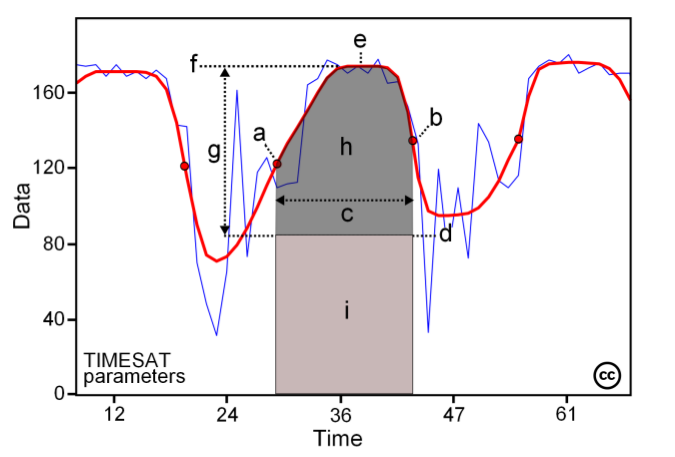
\includegraphics[scale=0.45]{synthese_biblio/metrics.png} 
 \end{center}
 \caption{Métriques phénologiques \citep{Eklundh2017} : a-SOS b-EOS c-Length of season d-Base value e-Middle of season f-Maximum NDVI g-Amplitude of NDVI}
 \label{metrics}
\end{figure}
%\clearpage
\vspace{5mm}

Outre leur utilisation comme proxy à l'évaluation des dates de semis, les métriques phénologiques peuvent être employées à d'autres fins comme l'estimation de rendements, exploitant 
la forte corrélation avec la biomasse en fin de saison ou encore la détection d'anomalies dans le cycle de la végétation, en considérant une référence ou une normale parmi un 
historique de saisons culturales.

\vspace{5mm}

Comme évoqué dans la \cref{general}, plusieurs méthodes ont été mises au point pour dériver les métriques phénologiques à partir de séries temporelles d'indices de végétation.
\citet{Atzberger2013} les a classé en 2 catégories : 
\begin{itemize}
 \item un premier groupe de méthodes qui estime les métriques phénologiques de manière indépendante à un instant donné 
 \item et un second groupe qui modélise le cycle entier par une fonction mathématique pour estimer les métriques phénologiques.
\end{itemize}

Dans le premier groupe, sont classées surtout les méthodes par seuillage des indices de végétation. Dans leur revue, \citet{deBeurs2010} en ont décrit quelques unes notamment le NDVI 
Ratios \citep{White1997}. Les méthodes par seuillage sont les plus simples et les plus communes \citep{Pan2015}. En effet, elles supposent qu’un stade phénologique a commencé quand 
la valeur de l'indice de végétation atteint un certain seuil fixé \citep{Jonsson2002}. Cependant, cette approche par seuillage peut s'avérer inconsistante quand le couvert n'est 
pas homogène. De plus, un seuil n'est pas toujours transposable du fait qu'il est bien souvent lié à sa zone d'application. La seconde catégorie regroupe  des méthodes comme
l'analyse de Fourier, la transformation en ondelettes, l'analyse en composantes principales ou encore les modèles logistiques. Ces dernières méthodes sont plus poussées et plus 
complexes à mettre en \oe uvre. 

\vspace{5mm}

Bon nombre de logiciels et applications ont été développés pour traiter les séries temporelles d'indices de végétation et en extraire les métriques phénologiques souhaitées. 
Nous avons identifié les suivants :
\begin{itemize}
 \item TIMESAT \footnote{\url{http://web.nateko.lu.se/timesat/timesat.asp?cat=0}} \citep{Eklundh2017} 
 \item SPIRITS \footnote{\url{http://spirits.jrc.ec.europa.eu/}}
 \item PhenoSat \footnote{\url{http://www.fc.up.pt/PhenoSat/software.html}} \citep{Rodrigues2013}
 \item Plugin QGIS QPhenoMetrics \citep{Duarte2018}
 \item Plugin QGIS VERSAO VegaMonitor \footnote{\url{https://github.com/Xdarii/VERSAO_VegaMonitor/wiki}}.
\end{itemize}

\section{Estimation des rendements par télédétection}


  \chapter{Matériels et Méthodes}
  
  \section{Présentation générale de la zone d'étude}

\section{Données satellitaires utilisées}

Notre série temporelle est composée de 3 types d’imageries satellitaires. Il s'agit d'images PlanetScope, RapidEye et Sentinel-2. 

  \subsection{Imageries PlanetScope et RapidEye}
  
Les images PlanetScope sont produites par la société privée américaine Planet Labs, Inc. \footnote{\url{https://www.planet.com/}}. Fondée en 2010 et basée à San Francisco 
en Californie, cette société est spécialisée dans l'observation de la terre par imagerie satellitaire. Planet Labs conçoit et fabrique des \emph{nanosatellites} ou \emph{CubSats} 
($10\times10\times30\,cm$) appelés \emph{Doves} qui sont placés sur orbite en tant que charge utile secondaire sur d'autres missions de lancement de fusée. La société dispose ainsi d'une
constellation de nanosatellites surnommée \emph{Flock}. La constellation est composée actuellement de 175 nanosatellites positionnés sur une orbite héliosynchorne à 475 km 
d’altitude. Ces nanosatellites produisent des images complètes de la Terre une fois par jour, à une résolution 
spatiale variant de 3 à 5 mètres. Ces images fournissent des informations permettant de suivre les changements climatiques, de prévoir les récoltes, de gérer les catastrophes ou encore de 
mettre au point des applications urbaines. Les images recueillies par les Doves sont accessibles en ligne et certaines disponibles dans le cadre de l'Open Data. \\
En 2015, Planet Labs a acquis la constellation RapidEye auprès de la société allemande BlackBridge. Les images RapidEye qui ont une résolution spatiale de 5 mètres sont fournies par une 
constellation de 5 satellites. Leur période de revisite est de 5 jours et demi au nadir ou journalière sinon. Enfin en 2017, Google a vendu sa filiale Terra Bella et sa constellation de 
satellites \emph{SkySat} à Planet Labs. Les images SkySat ont une résolution submétrique (80 cm). 

    \paragraph{Spécifications des images PlanetScope}

Trois niveaux de traitements sont disponibles pour les images PlanetScope. Ce sont les niveaux 1B, 3A et 3B. Le niveau 1B correspond aux produits basiques. Les données numériques ont 
été calibrées en radiance \acrshort{toa} mais les images ne sont pas géoréférencées. Le niveau 3B qui est celui de nos images correspond à des produits orthorectifiés et projetés en
\acrshort{utm}. Comme pour le niveau 1B, les valeurs numériques ont été calibrées en radiance TOA. Le niveau 3A est similaire au 3B à la différence que les images sont tuilées pour 
couvrir un système de grilles de $25\times25$ kilomètres.\\
Les images PlanetScope sont distribuées en format \emph{GeoTiff}. Au niveau 3B, elles ont une résolution au sol de \emph{3 mètres} et une résolution radiométrique de \emph{12 bits} s'il 
s'agit de compte numérique ou \emph{16 bits} dans le cas des radiances TOA. Elles disposent de 4 bandes spectrales (\Cref{planetscope}). 

\begin{table}[htbp]
\begin{center}
\caption{Caractéristiques spectrales des images PlanetScope}
\label{planetscope}
 \begin{tabular}{ccc}
  \hline
  Bande spectrale & Domaine spectral & Longueurs d'onde (\SI{}{\micro\meter})\\
  \hline
  1 & Bleu & 0,455 --- 0,515 \\
  2 & Vert & 0,500 --- 0,590 \\
  3 & Rouge & 0,590 --- 0,670 \\
  4 & Proche Infrarouge & 0,780 --- 0,860 \\ 
  \hline
 \end{tabular}
\end{center}
\end{table}

La conversion des données PlanetScope en réflectance TOA s'effectue par la formule suivante :
\begin{align}
   Reflectance (i) = DN(i) \times reflectanceFactor(i)
\end{align}

où :\\
\emph{i} = Numéro de la bande spectrale de l'image,\\
\emph{DN} = Valeurs numériques (brutes) de l'image,\\
et \emph{reflectanceFactor(i)} = Facteur de conversion en réflectance pour une bande spectrale donnée, renseigné dans les metadonnées de l'image.

  \paragraph{Spécifications des images RapidEye}

Les images RapidEye sont pour leur part, disponibles en 2 niveaux de traitements : 1B et 3A. Ces niveaux de traitements sont identiques à ceux des produits PlanetScope. Les images
RapidEye utilisées sont traitées au niveau 3A. Elles sont distribuées également en format \emph{GeoTiff}. Leur résolution au sol est de \emph{5 mètres} et leur résolution 
radiométrique de \emph{16 bits}. Elles disposent de 5 bandes spectrales (\Cref{rapideye}).

\begin{table}[htbp]
\begin{center}
\caption{Caractéristiques spectrales des images RapidEye}
\label{rapideye}
 \begin{tabular}{ccc}
  \hline
  Bande spectrale & Domaine spectral & Longueurs d'onde (\SI{}{\micro\meter})\\
  \hline
  1 & Bleu & 0,440 --- 0,510 \\
  2 & Vert & 0,520 --- 0,590 \\
  3 & Rouge & 0,630 --- 0,685 \\
  4 & Red Edge & 0,690 --- 0,730 \\ 
  5 & Proche Infrarouge & 0,760 --- 0,850 \\
  \hline
 \end{tabular}
\end{center}
\end{table}

La conversion des données RapidEye en réflectance TOA s'effectue en 2 étapes à savoir la conversion en radiance puis la conversion en réflectance :

\begin{align} Radiance (i) = &  DN(i) \times radiometricScaleFactor(i) \\
Reflectance(i) = &  Radiance(i) \times \frac{\pi \times SunDist^2}{EAI(i) \times \cos(SolarZenith)} 
\end{align}

où :\\
\emph{i} = Numéro de la bande spectrale de l'image \\
\emph{DN} = Valeurs numériques (brutes) de l'image \\
\emph{radiometricScaleFactor(i)} = Facteur de conversion en radiance pour une bande spectrale donnée, renseigné dans les métadonnées de l'image \\
\emph{SunDist} = Distance Terre-Soleil en unités astronomiques \\
\emph{EAI(i)} = Irradiance exo-atmosphérique pour une bande spectrale donnée, renseignée dans les métadonnées de l'image \\
\emph{SolarZenith} = Angle zénithal solaire en degrés (90\textdegree - Elévation solaire)

  \subsection{Imagerie Sentinel-2}

Sentinel est une famille de 6 satellites d'observation de la Terre, développée par l'\acrshort{esa} et destinée à assurer la continuité des données de la mission \acrshort{envisat} arrivée à 
terme en 2012. Sentinel représente le volet spatial du programme Copernicus (ex \acrshort{gmes}) de l'Union Européenne qui vise à doter l'Europe d'une capacité autonome et 
opérationnelle en matière d'observation de la Terre notamment pour la surveillance de l'environnement et la sécurité \citep{Drusch2012}. La mission Sentinel-2 est la composante spatiale du programme 
devant fournir une imagerie optique haute résolution permettant l’observation des sols (utilisation, végétation, zones côtières, fleuves \ldots) ainsi que la mise en place de services 
de traitement des situations d'urgence notamment les catastrophes naturelles. Cette mission est composée des satellites \emph{Sentinel-2A} et \emph{Sentinel-2B} qui circulent
en déphasage de 180\textdegree{} sur la même orbite héliosynchrone de 10h30. Ces 2 satellites sont identiques et embarquent l'instrument \acrshort{msi} qui fournit des images dans 13 bandes spectrales 
du Visible à l'Infrarouge (\Cref{msi}) avec une résolution spatiale comprise entre 10 et 60 mètres et une résolution radiométrique de 12 bits. Les satellites Sentinel-2 sont configurés pour une période 
de revisite de 5 jours au nadir et doivent acquérir au moins une donnée claire par mois sur la plupart des terres émergées. 
Cette grande richesse spectrale couplée à cette capacité d'observation temporelle élevée constituent le véritable apport de la mission Sentinel-2. Les données sont principalement 
utilisées pour l'agriculture, la sylviculture, l'occupation des sols, la biodiversité, la caractérisation des habitats ou encore l'observation et la prévention des catastrophes 
naturelles notamment les inondations. 

\begin{table}[htbp]
\begin{center}
\caption{Caractéristiques spectrales de l'instrument MSI des Sentinel-2}
\label{msi}
 \begin{tabular}{cccc}
  \hline
  Bande spectrale & Domaine spectral & Longueurs d'onde (\SI{}{\micro\meter}) & R. spatiale (m)\\
  \hline
  \phantom{1}1 & Aérosols & 0,433 --- 0,453 & 60 \\
  \phantom{1}2 & Bleu & 0,4575 --- 0,5225 & 10 \\
  \phantom{1}3 & Vert & 0,5425 --- 0,5775 & 10 \\
  \phantom{1}4 & Rouge & 0,65 --- 0,68 & 10 \\ 
  \phantom{1}5 & Red Edge & 0,6975 --- 0,7125 & 20 \\
  \phantom{1}6 & Red Edge & 0,7325 --- 0,7475 & 20 \\
  \phantom{1}7 & Red Edge & 0,773 --- 0,793 & 20 \\
  \phantom{1}8 & Proche Infrarouge & 0,83625 --- 0,84775 & 10\\
  8A & Red Edge & 0,855 --- 0,875 & 20 \\
  \phantom{1}9 & Vapeur d'eau & 0,935 --- 0,955 & 60 \\
  10 & Cirrus & 1,365 --- 1,395 & 60 \\
  11 & Infrarouge moyen & 1,565 --- 1,655 & 20 \\
  12 & Infrarouge moyen & 2,181 --- 2,199 & 20 \\
  \hline
 \end{tabular}
\end{center}
\end{table}

Les images Sentinel-2 utilisées dans ce travail sont produites par \acrshort{theia}/\acrshort{muscate} \footnote{\url{http://www.theia-land.fr/}}. Il s'agit de données Copernicus 
Sentinel-2 de niveau 1C (données ortho-rectifiées en réflectance TOA) qui sont traités au niveau 2A (données ortho-rectifiées en réflectance de surface après correction atmosphérique
notamment par \acrshort{maccs}/\acrshort{maja} \footnote{\url{http://www.cesbio.ups-tlse.fr/multitemp/?p=6050}}). Au niveau 2A, des masques de nuages et d'ombres ainsi que 
des surfaces d’eau et de neige sont fournis. Les données de réflectance fournies sont de 2 types :
\begin{itemize}
 \item le SRE pour Surface REflectance qui incluent les corrections atmosphériques et effets d'environnement
 \item le FRE pour Flat REflectance qui incluent en plus des corrections des données SRE, les corrections liées aux effets de pente.
\end{itemize}
Notons qu'à terme, seules les données FRE seront fournis par Theia, afin de diminuer les volumes à distribuer. 

\vspace{5mm}

Nos images Sentinel-2 sont des données SRE. Elles sont codées en entiers sur du 16 bits signé. L'obtention des vraies valeurs de réflectance est donnée par :
\begin{align}
  Reflectance (i) =  \frac{ReflectanceCodee(i)}{10\,000}
\end{align}

\vspace{5mm}
 
Nous avons mis en place une chaîne de prétraitements, écrite avec le langage de programmation \texttt{Python}, pour effectuer la calibration de nos images en données de 
réflectance (TOA pour les images PlanetScope et RapidEye et réflectance de surface pour les images Sentinel-2) et leur découpage selon l'emprise de notre zone d'étude. 
Les bibliothèques \texttt{gdal} et \texttt{rasterio} ont été utilisées à cet effet. Notons que pour les images PlanetScope et certaines images RapidEye, nous avons d'abord dû 
effectuer un mosaiquage de toutes les images correspondant à la même date d'acqusition avant de les découper. Pour leur part, les bandes Red Edge des images Sentinel-2 (20 mètres 
de résolution) ont été rééchantillonnées à 10 mètres et empilées avec les bandes originelles de 10 mètres. Les bandes de 60 mètres qui sont plus relatives aux applications 
météorologiques n'ont pas été considérées dans le cadre de ce stage.

  \subsection{Chronologie des images acquises}
  
Les 27 images utilisées ont été acquises entre Juin et Novembre 2017, période couvrant la saison agricole 2017. Cependant, nous ne disposons que d'une image (PlanetScope) en Septembre. La 
Chronologie des acquisitions (\Cref{Chronologie}) est la suivante :

\begin{figure}[htbp]
  \begin{center}
    \begin{tikzpicture}
     \begin{axis}[hide y axis,axis lines=middle,
      date coordinates in=x,
      xticklabel={\texttt{\month}},
      xlabel=RapidEye,
      xlabel style={at={(current axis.right of origin)}, xshift=7.5ex, anchor=center},
      %x tick label style={},
      date ZERO=2017-05-01,
      xmin=2017-05-25,
      xmax=2017-12-05,
      ymin=0,ymax=0.1,
      xtick=\empty,clip=false]
      \addplot [magenta,thick,mark=*,only marks]coordinates{
        (2017-07-27,0)
        (2017-10-06,0)
        (2017-10-26,0)
        (2017-11-09,0)
        };
      \end{axis}
  \end{tikzpicture}
  
  \begin{tikzpicture}
    \begin{axis}[hide y axis,axis lines=middle,
      date coordinates in=x,
      xticklabel={\texttt{\month}},
      xlabel=Sentinel-2,
      xlabel style={at={(current axis.right of origin)}, xshift=7.5ex, anchor=center},
      %x tick label style={},
      date ZERO=2017-05-01,
      xmin=2017-05-25,
      xmax=2017-12-05,
      ymin=0,ymax=0.1,
      xtick=\empty,clip=false]
      \addplot [magenta,thick,mark=*,only marks]coordinates{
        (2017-06-07,0)
        (2017-06-17,0)
        (2017-07-27,0)
        (2017-08-06,0)
        (2017-10-05,0)
        (2017-10-15,0)
        (2017-10-25,0)
        (2017-11-04,0)
        (2017-11-14,0)};
     \end{axis}
    \end{tikzpicture}
  
  \begin{tikzpicture}
    \begin{axis}[hide y axis,axis lines=middle,
      date coordinates in=x,
      xticklabel={\texttt{\month}},
      xlabel={PlanetScope},
      xlabel style={at={(current axis.right of origin)}, xshift=7.5ex, anchor=center},
      %x label style={},
      date ZERO=2017-05-01,
      xmin=2017-05-25,
      xmax=2017-12-05,
      ymin=0,ymax=0.1,
      xtick={{2017-06-01},{2017-07-01},{2017-08-01},{2017-09-01},{2017-10-01},{2017-11-01},{2017-12-01}},clip=false]
      \addplot [magenta,thick,mark=*,only marks]coordinates{
        (2017-06-04,0)
        (2017-06-18,0)
        (2017-07-09,0)
        (2017-07-16,0)
        (2017-07-27,0)
        (2017-08-15,0)
        (2017-09-19,0)
        (2017-10-01,0)
        (2017-10-11,0)
        (2017-10-16,0)
        (2017-10-23,0)
        (2017-10-30,0)
        (2017-11-15,0)
        (2017-11-19,0)};
    \end{axis}
   \end{tikzpicture}
   
  \end{center}
  \caption{Chronologie des images acquises}
  \label{Chronologie}
\end{figure}

\section{Données de terrain}

Notre jeu de données terrain est basé sur des enquêtes agronomiques réalisées courant 2017 sur 53 parcelles agricoles. Ces enquêtes ont été menées pour la plupart dans le cadre des projets Oracle \footnote{\url{https://afrique-ouest.cirad.fr/actualites/projet-oracle-2017-2020}} et ANR CERAO \footnote{\url{http://www.agence-nationale-recherche.fr/Projet-ANR-13-AGRO-0002}}. Le jeu du projet Oracle provient de la thèse de Sophie \textsc{Djiba} et consiste en un réseau de 30 parcelles enquêtées en milieu paysan où les pratiques agricoles sont 
axées sur des rotations entre céréales et légumineuses (mil/arachide et/ou niébé) et des associations entre légumineuses (arachide/niébé). Par contre, celui du projet ANR CERAO, mis au point par Adama \textsc{Tounkara} lors de sa thèse, est un réseau de 19 parcelles enquêtées également en milieu paysan mais présentant chacune sur une partie, des essais relatifs à l'efficience de l'utilisation de l'azote par le mil en fonction de différents niveaux d'apports ou non en fertilisants, et ce indépendamment des pratiques de l'agriculteur. Nous émettons l'hypothèse que ces essais sont représentatifs des parcelles concernées, néanmoins, conscients de l'incertitude potentielle dans cette généralisation, nous envisageons d'analyser nos résultats séparement en tenant compte de la source des données de terrain. Pour chaque parcelle enquêtée, différentes informations sont collectées. Celles qui nous interessent principalement sont :
\begin{itemize}
 \item le système de culture et les espèces cultivées
 \item les pratiques culturales (fertilisant, dates de semis et de récoltes)
 \item la biomasse (fraîche et sèche) et le rendement (frais et sec)
 \item la géolocalisation des parcelles
 \item ou encore le nombre et les espèces d'arbres présentes au sein des parcelles.
\end{itemize}
La \Cref{terrain} présente les principales statistiques descriptives pour les parcelles enquêtées. Comme nous pouvons nous en apercevoir \ldots{} comme espéré. La \ldots{} présente la localisation des parcelles suivant leur culture et système de culture ainsi que leur biomasse fraîche et les rendements frais observés.

\begin{table}[htbp]
%\begin{center}
\caption{Statistiques descriptives des données de terrain}
\label{terrain}
 \begin{tabular}{ccccc}
  \hline
  Culture majoritaire & Système de culture & Nombre de parcelles & Biomasse fraiche (kg/ha) & Rendement frais (kg/ha)\\
  \hline
  Arachide & Mixte & 19 & 0 & 0 \\
  Mil & Pure & 19 & 0 & 0 \\
  Mil & Mixte & 19 & 0 & 0 \\
  \hline
 \end{tabular}
%\end{center}
\end{table}


  
\section{Extraction d'indices spectraux}

Sur base des images de réflectance, nous avons extrait 2 indices de végétation. Il importe de noter que les indices dérivés d'images RapidEye (5m) ou Sentinel-2 (10m) 
ont été rééchantillonnés à la résolution des indices PlanetScope (3m), ce afin de pouvoir considérer une série temporelle par indice calculé. 

\paragraph{NDVI} \citep{Rouse1974,Tucker1979} 

\begin{align}
 NDVI = \frac{PIR - R}{PIR + R}
\end{align}

\paragraph{MSAVI2} \citep{Qi1994}

\begin{align}
 MSAVI2 = \frac{2 \times (PIR + 1) - \sqrt{((2 \times PIR + 1)^2 - 8 \times (PIR - R))}}{2}
\end{align}

\section{Lissage des séries temporelles}

\`A présent que nous disposons d'une série temporelle pour chaque indice de végétation calculé, nous pouvons les exploiter pour la suite de notre travail. Cependant, un autre traitement s'impose : le \emph{lissage} ou \emph{smoothing}. En effet, bien que des prétraitements soient effectués sur les images satellitaires : calibrations radiométriques et corrections atmosphériques entre autres, il subsiste du bruit qui affecte l'utilisation des séries temporelles d'images, impactant ainsi les futures analyses et pouvant donc fausser les interprétations données aux résultats obtenus \citep{Chen2004}. Ce bruit résiduel peut être lié à plusieurs facteurs notamment les conditions atmosphériques variables ou la présence de pixels nuageux indétectés. Les techniques de lissage font l'hypothèse que le bruit résiduel dans les images entraine des chutes soudaines dans le profil temporel des indices de végétation \citep{Bojanowski2009}. Ces valeurs peuvent être ainsi identifiées puis supprimées et des séries temporelles de meilleure qualité reconstruites.
\\L'une des techniques usuelles adoptée notamment par les fournisseurs d'indices de végétation périodique comme GIMMS-MODIS, SPOT-VEGETATION ou PROBA-V est le \acrshort{mvc} \citep{Holben1986}. Cette technique 
consiste à créer des synthèses d'indices de végétation sur une période donnée, généralement une décade en considérant pour chaque pixel la plus grande valeur enrégistrée sur la période.
D'autres techniques de lissage de séries temporelles d'indices de végétation ont été mises au point. Nous pouvons citer des méthodes par seuillage comme les algorithmes \acrshort{bise} \citep{Viovy1992} ou \acrshort{idr} \citep{Julien2010} qui utilisent un seuil pour contrôler le degré de lissage des séries reconstruites, des méthodes qui définissent un filtre pour lisser les données dans une fenêtre mobile comme le filtre de Savitzky-Golay \citep{Savitzky1964, Chen2004} ou le filtre à poids variable de \citet{Zhu2012} ou encore d'autres méthodes qui ajustent des fonctions mathématiques au profil saisonnier de la végétation telles que la fonction asymétrique gaussienne \citep{Jonsson2002}, les doubles fonctions logistiques \citep{Beck2006} et les méthodes basées sur l'analyse de Fourier comme \acrshort{hants} \citep{Verhoef1996, Roerink2000} et la transformée de Fourier rapide \citep{Menenti1993}. La méthode de lissage de Whittaker \citep{Eilers2003,Atzberger2011} et la transformation en ondelettes \citep{Lu2007} sont également d'autres approches existantes.
\\Plusieurs études ces dernières années ont comparé différentes techniques de lissage \citep{Jonsson2002,Chen2004,Hird2009,Kandasamy2013,Geng2014,Shao2016,Liu2017} et beaucoup ont conclu qu'il n'y avait pas de méthode de lissage idéale, chacune présentant ses avantages et inconvénients. C'est notamment le cas de \citet{Geng2014} qui ont comparé pas moins de 8 méthodes de lissage pour reconstruire des séries temporelles de NDVI. De plus, la comparaison entre les méthodes de lissage n'est pas toujours significative du fait de l'objet de l'étude (simple comparaison, classification \ldots{}), des différentes données utilisées et de l'application à des zones parfois caractérisées par des facteurs environnementaux opposés. 
Néanmoins, s'il est vrai qu'aucun classement absolu des méthodes de lissage n'ait été établi, il n'en demeure pas moins que certaines méthodes reviennent souvent dans la littérature et ont donné de bons résultats. Le filtre de Savitzky-Golay notamment est connu pour ses résultats consistants \citep{Chen2004,Bojanowski2009,Kandasamy2013,Kim2014,Geng2014} et apprécié comme l'une des méthodes de lissage qui conserve le mieux la forme du profil temporel des indices de végétation ainsi que le timing et l'amplitude des minima et maxima locaux \citep{Geng2014}. L'algorithme HANTS a également été utilisé avec succès à de nombreuses reprises pour reconstruire des séries temporelles d'indices de végétation comme le NDVI ou de température de surface \citep{Roerink2000,Jakubauskas2001,Lunetta2006,Julien2006,Zhou2012,Zhou2015}. HANTS a été particulièrement développé pour traiter les séries temporelles d'observations irrégulièrement espacées dans le temps, identifier et supprimer les observations nuageuses \citep{Verhoef1996,Roerink2000} et prédire les observations manquantes. Ces points siéent parfaitement aux caractéristiques de nos séries temporelles. Par ailleurs, \citet{Atzberger2011} a montré que la méthode de lissage de Whittaker pouvait parfaitement faire l'équilibre entre fidélité aux données d'origine et lissage tout en restant facile à mettre en oeuvre et en permettant un traitement rapide des données \citep{Eilers2003}. \citet{Atkinson2012,Geng2014,Shao2016} ont également démontré les bonnes performances de cette méthode. Pour les raisons citées, nous avons donc retenu et comparé ces 3 approches pour lisser nos séries temporelles.

\subsection{Filtre de Savitzky-Golay}

\subsection{HANTS}

HANTS est un algorithme fondé sur l'analyse harmonique qui est une branche des mathématiques étudiant la représentation des fonctions ou signaux comme une superposition de fonctions périodiques. L’analyse en harmonique décompose le signal en une somme de fonctions sinusoïdales. Quand elle est utilisée pour reconstruire une série temporelle d’observations satellitaires, la série reconstruite \tilde{y} s’écrit :

\begin{align}   
    \tilde{y}(t_{j}) = a_{0} + \sum_{i=1}^{n_{f}} a_{i}\cos(2\pi f_{i} t_{j}) + b_{i}\sin(2\pi f_{i} t_{j})
\end{align}

\begin{align}
 y(t_{j}) = \tilde{y}(t_{j}) + \varepsilon(t_{j})
\end{align}

où : \\
$y$ est la série temporelle d’origine, $\varepsilon$ les erreurs résiduelles, $t_{j}$ le temps où y est observé
dans la série temporelle $(t_{1}, t_{2}, \ldots{} t_{N} )$ avec $N$ comme nombre maximal d’échantillons dans
la série temporelle; $n_{f}$ est le nombre de termes périodiques dans la série temporelles ou
le nombre d’harmoniques associées à la fréquence $f_{i}$. $a_{i}$ et $b_{i}$ sont les c\oe fficients des
composantes trigonométriques de la fréquence $f_{i}$. $a_{0}$ est le c\oe fficient à la fréquence zéro (phase nulle) et représente la moyenne de la série \citep{Zhou2015}.


\subsection{Méthode de lissage de Whittaker}

\subsection{Evaluation du lissage}

surtout couvrir le Mois de septembre qui a une seule image

\section{Extraction des Métriques Phénologiques}

\section{Estimation des Rendements}


  \chapter{Résultats et Discussions}
  
  \section{Résultats}

\subsection{Extraction du SOS et du EOS}

\`A partir des profils temporels de NDVI obtenus par les 2 méthodes de lissage (HANTS et Whittaker), nous avons extrait le SOS et le EOS respectivement avec les seuils de 10, 20, 30 puis 50\% avant le MAX et 50, 60, 70 puis 80\% après le MAX. Nous avons calculé ensuite pour chacune des parcelles terrain, les écarts en nombre de jours entre les dates de semis et les SOS extraits puis entre les dates de récolte et les EOS estimés. En considérant ces écarts par sytème de culture, nous avons calculé 2 indicateurs statistiques : la racine carrée de l'erreur quadratique moyenne ou \acrshort{rmse} qui est un indicateur d'écart entre valeurs observées et valeurs prédites et le coefficient de variation ou \acrshort{cv} qui mesure la dispersion relative autour la moyenne. 

\paragraph{SOS et évaluation des dates de semis}
La distribution des écarts entre les dates de semis observées et les SOS extraits par système de culture et méthode de lissage est illustrée sur la \cref{fig-sosboxplot}. Globalement, les parcelles d'arachide mixte montrent les variabilités les plus faibles entre les écarts calculés (moins de 15 jours d'écart au maximum, seuils et méthodes de lissage confondus) suivies des parcelles de mil pur (moins de 20 jours d'écart au maximum, seuils et méthodes de lissage confondus) et des parcelles de mil mixte qui présentent les variabilités les plus fortes (près de 60 jours d'écart avec les SOS estimés par HANTS pour un seuil de 10\%). En analysant la distribution des écarts par méthode de lissage, nous remarquons que pour l'ensemble des systèmes de culture et presque pour tous les seuils, la plage des écarts obtenus avec les SOS estimés par HANTS est toujours plus importante que celle des écarts obtenus avec les SOS extraits par la méthode de Whittaker avec des écarts plus grands pour HANTS quand on considère le même seuil. Ceci semble indiquer que la méthode de lissage de Whittaker soit plus appropriée pour estimer le timing du démarrage de croissance de la végétation. L'analyse de la distribution des écarts en fonction du seuil d'extraction du SOS montre quant à elle une certaine tendance à la réduction de la variabilité des écarts quand le seuil d'extraction s'accroit, méthodes de lissage et systèmes de culture confondus à l'exception du mil pur. Cependant, cette tendance est à relativiser au vu de l'apparition de valeurs aberrantes à mesure que le seuil d'extraction du SOS croît et d'autant plus que les écarts entre dates de semis et SOS estimés s'accroissent également, ce qui est tout à fait logique puisque l'amplitude du NDVI avant le MAX est proportionnelle au temps. En effet, plus ces écarts seront importants et plus les SOS déterminés ne seront plus réalistes vis-à-vis du temps de germination des semences, l'inverse étant également vraie. 
Ainsi, nous pouvons remarquer que le seuil de 10\% extrait parfois des SOS précoces (écarts 
négatifs pour certaines parcelles d'arachide et de mil mixtes) et que le seuil de 50\% les extrait tardivement (40 à 60 jours après les dates de semis). Le seuil le plus adapté doit extraire les SOS avec des écarts réalistes par rapport aux dates de semis et minimiser au mieux la variabilité entre ces écarts. Afin de déterminer les seuils les plus adaptés et ce par système de culture, référons nous à la \cref{fig-sos-rmse-cv} où nous avons représenté le RMSE entre les dates de semis et SOS estimés en fonction du coefficient de variation (CV) de leurs écarts par système de culture et méthode de lissage. La variation du RMSE en fonction du seuil d'extraction  quelque soit le système de culture ou la méthode de lissage pris en compte rejoint l'analyse sur la distribution des écarts. En effet, plus le seuil d'extraction croit et plus le RMSE entre SOS et dates de semis est grand, ce dernier étant un indicateur d'écart. La variation du CV en fonction du seuil d'extraction révèle d'abord 2 valeurs qui portent à interrogation : -233\% (pour un seuil de 10\% avec la méthode de Whittaker sur les parcelles d'arachide mixte) et 342\% (pour un seuil de 10\% avec HANTS sur les parcelles de mil mixte). Notre investigation a révélé qu'il s'agissait de cas où l'écart-type était supérieure à une moyenne très petite  proche de $0$ (négative et positive respectivement). Ceci indique que les SOS extraits dans ces cas sont précoces. Pour le reste, la valeur du coefficient de variation diminue quand le seuil d'extraction croît, système de culture et méthode de lissage confondus. Ceci peut s'expliquer par le fait que la moyenne des écarts entre SOS et dates de semis augmente à mesure que le seuil d'extraction s'accroit quand l'écart-type ou la variabilité entre les écarts est sensiblement la même. Finalement, il apparait que le seuil le plus adapté pour les parcelles d'arachide mixte est celui de 20\% avec la méthode de Whittaker qui estime les SOS avec un RMSE légèrement supérieur à 10 jours. Pour les parcelles de mil pur et de mil mixte, le seuil de 10\% avec la méthode de Whittaker apparait être le plus adapté avec des RMSE de 15 jours sur les estimations de SOS. Nous avons également spatialisé les SOS extraits (\Cref{fig-spatial-sos}).
\begin{figure}[htbp]
 \begin{center}
  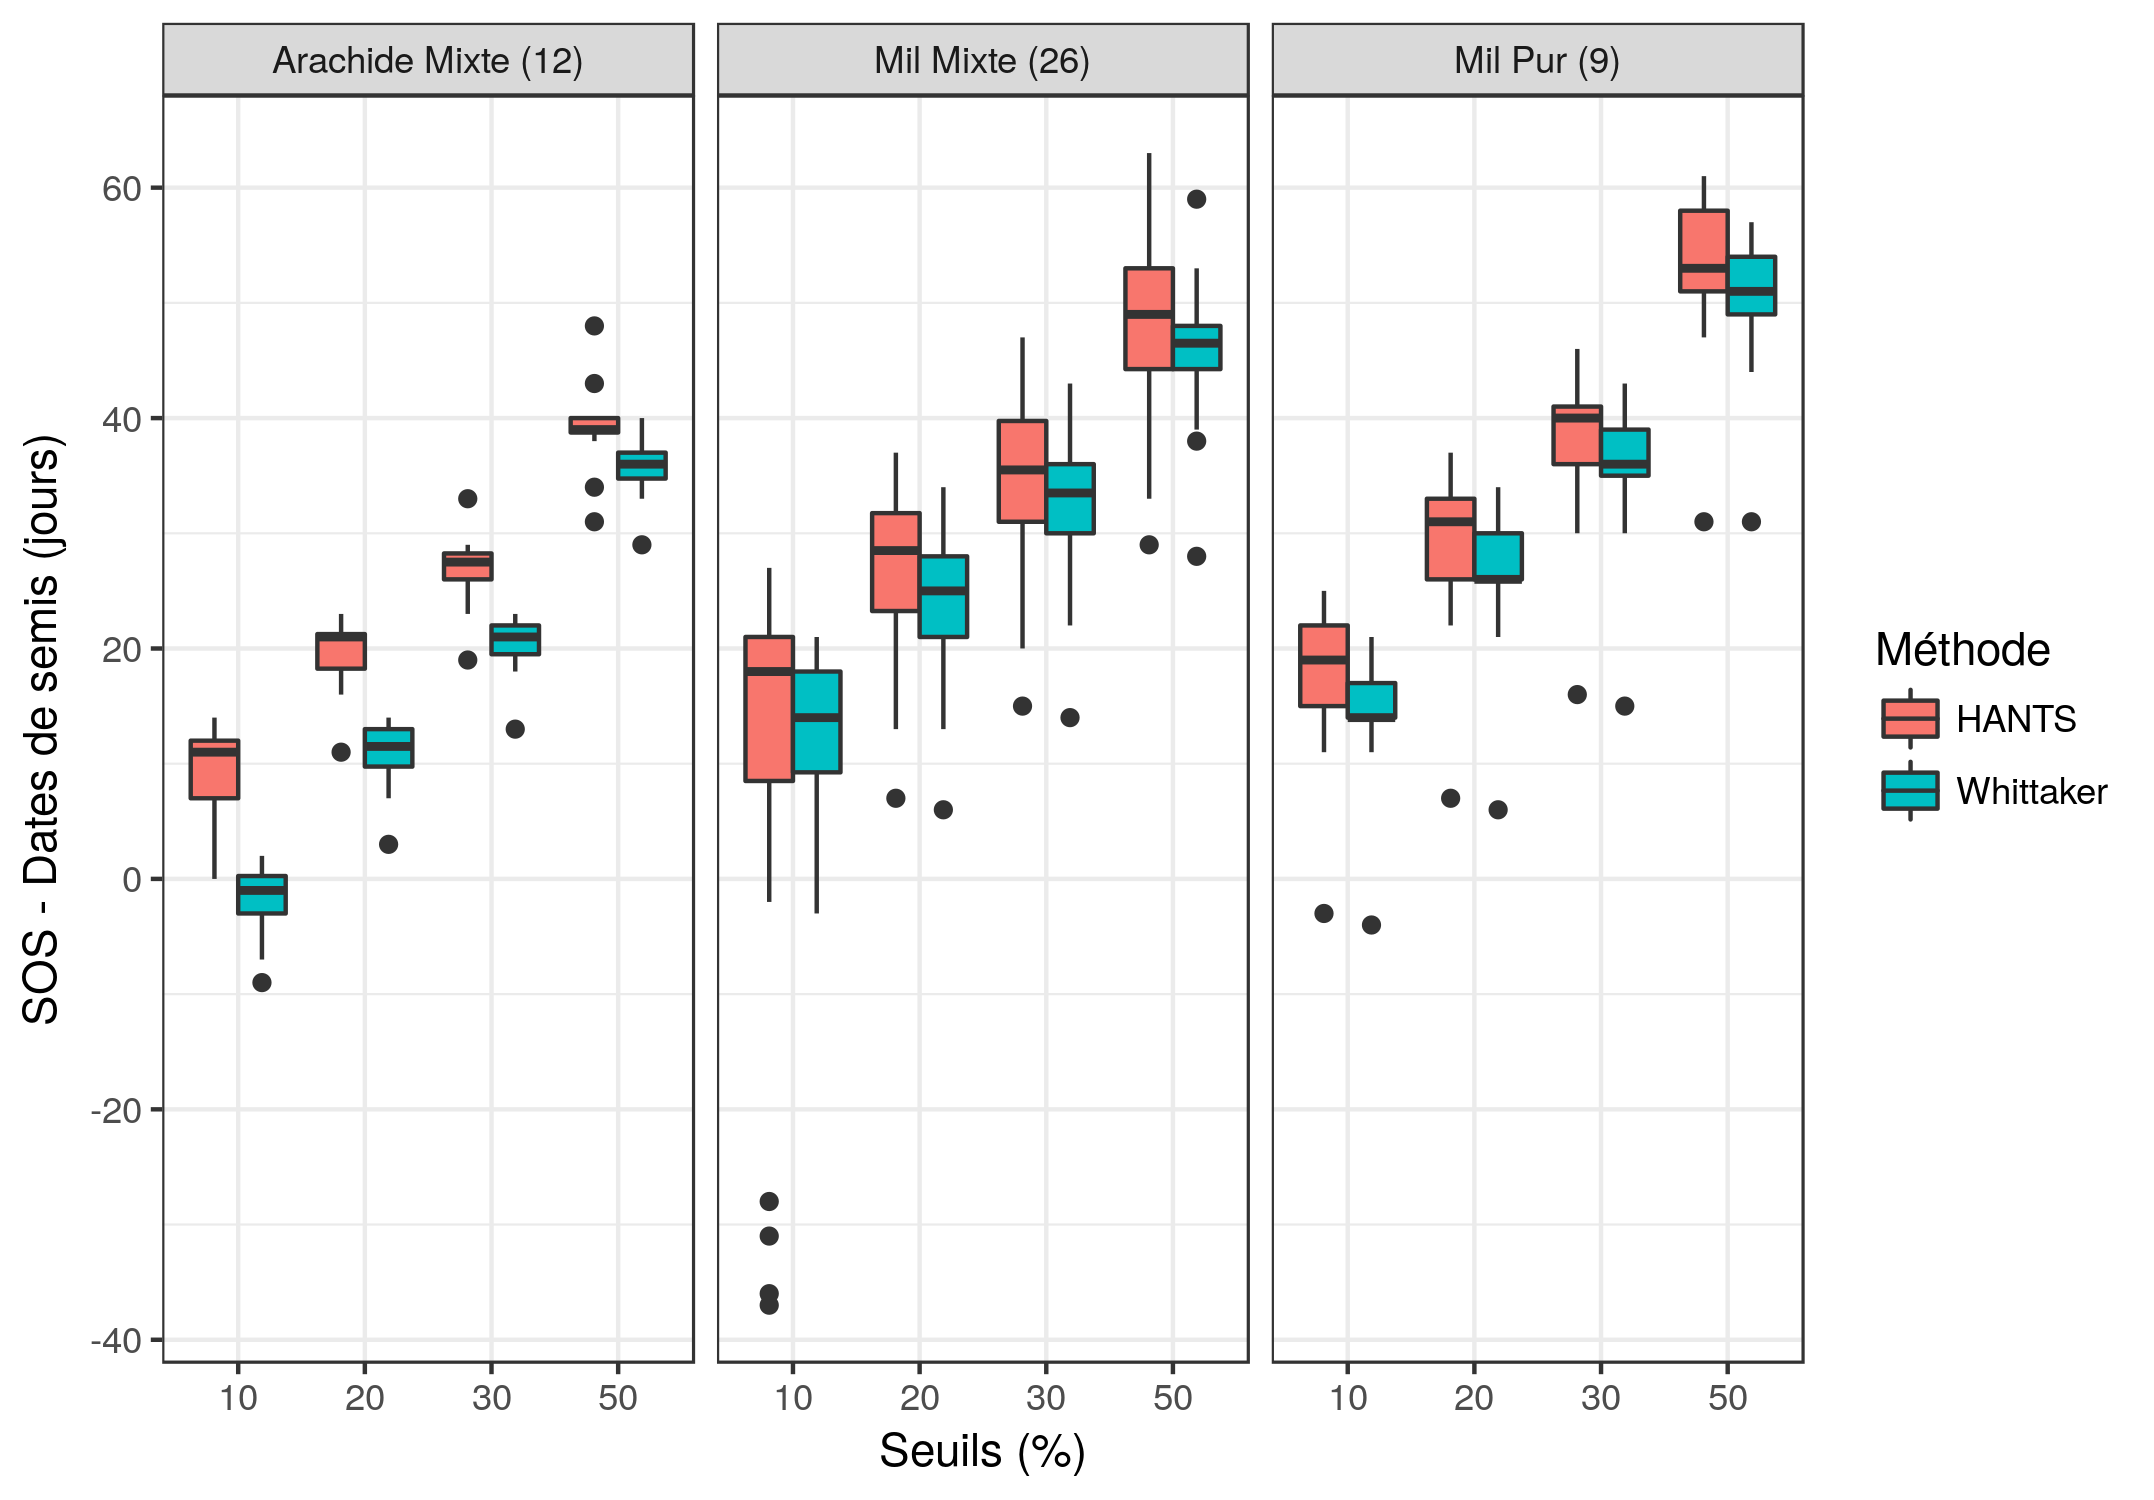
\includegraphics[scale=0.7]{resultats_discussions/SOS_Boxplot.png} 
 \end{center}
 \caption[Distribution des écarts entre SOS et dates de semis]{Boîtes à moustaches illustrant la distribution des écarts entre SOS estimés et dates de semis observées en fonction des systèmes de culture et des méthodes de lissage (\emph{Le nombre de parcelles est indiqué à la suite du système de culture})}
 \label{fig-sosboxplot}
\end{figure}

\begin{figure}[htbp]
 \begin{center}
  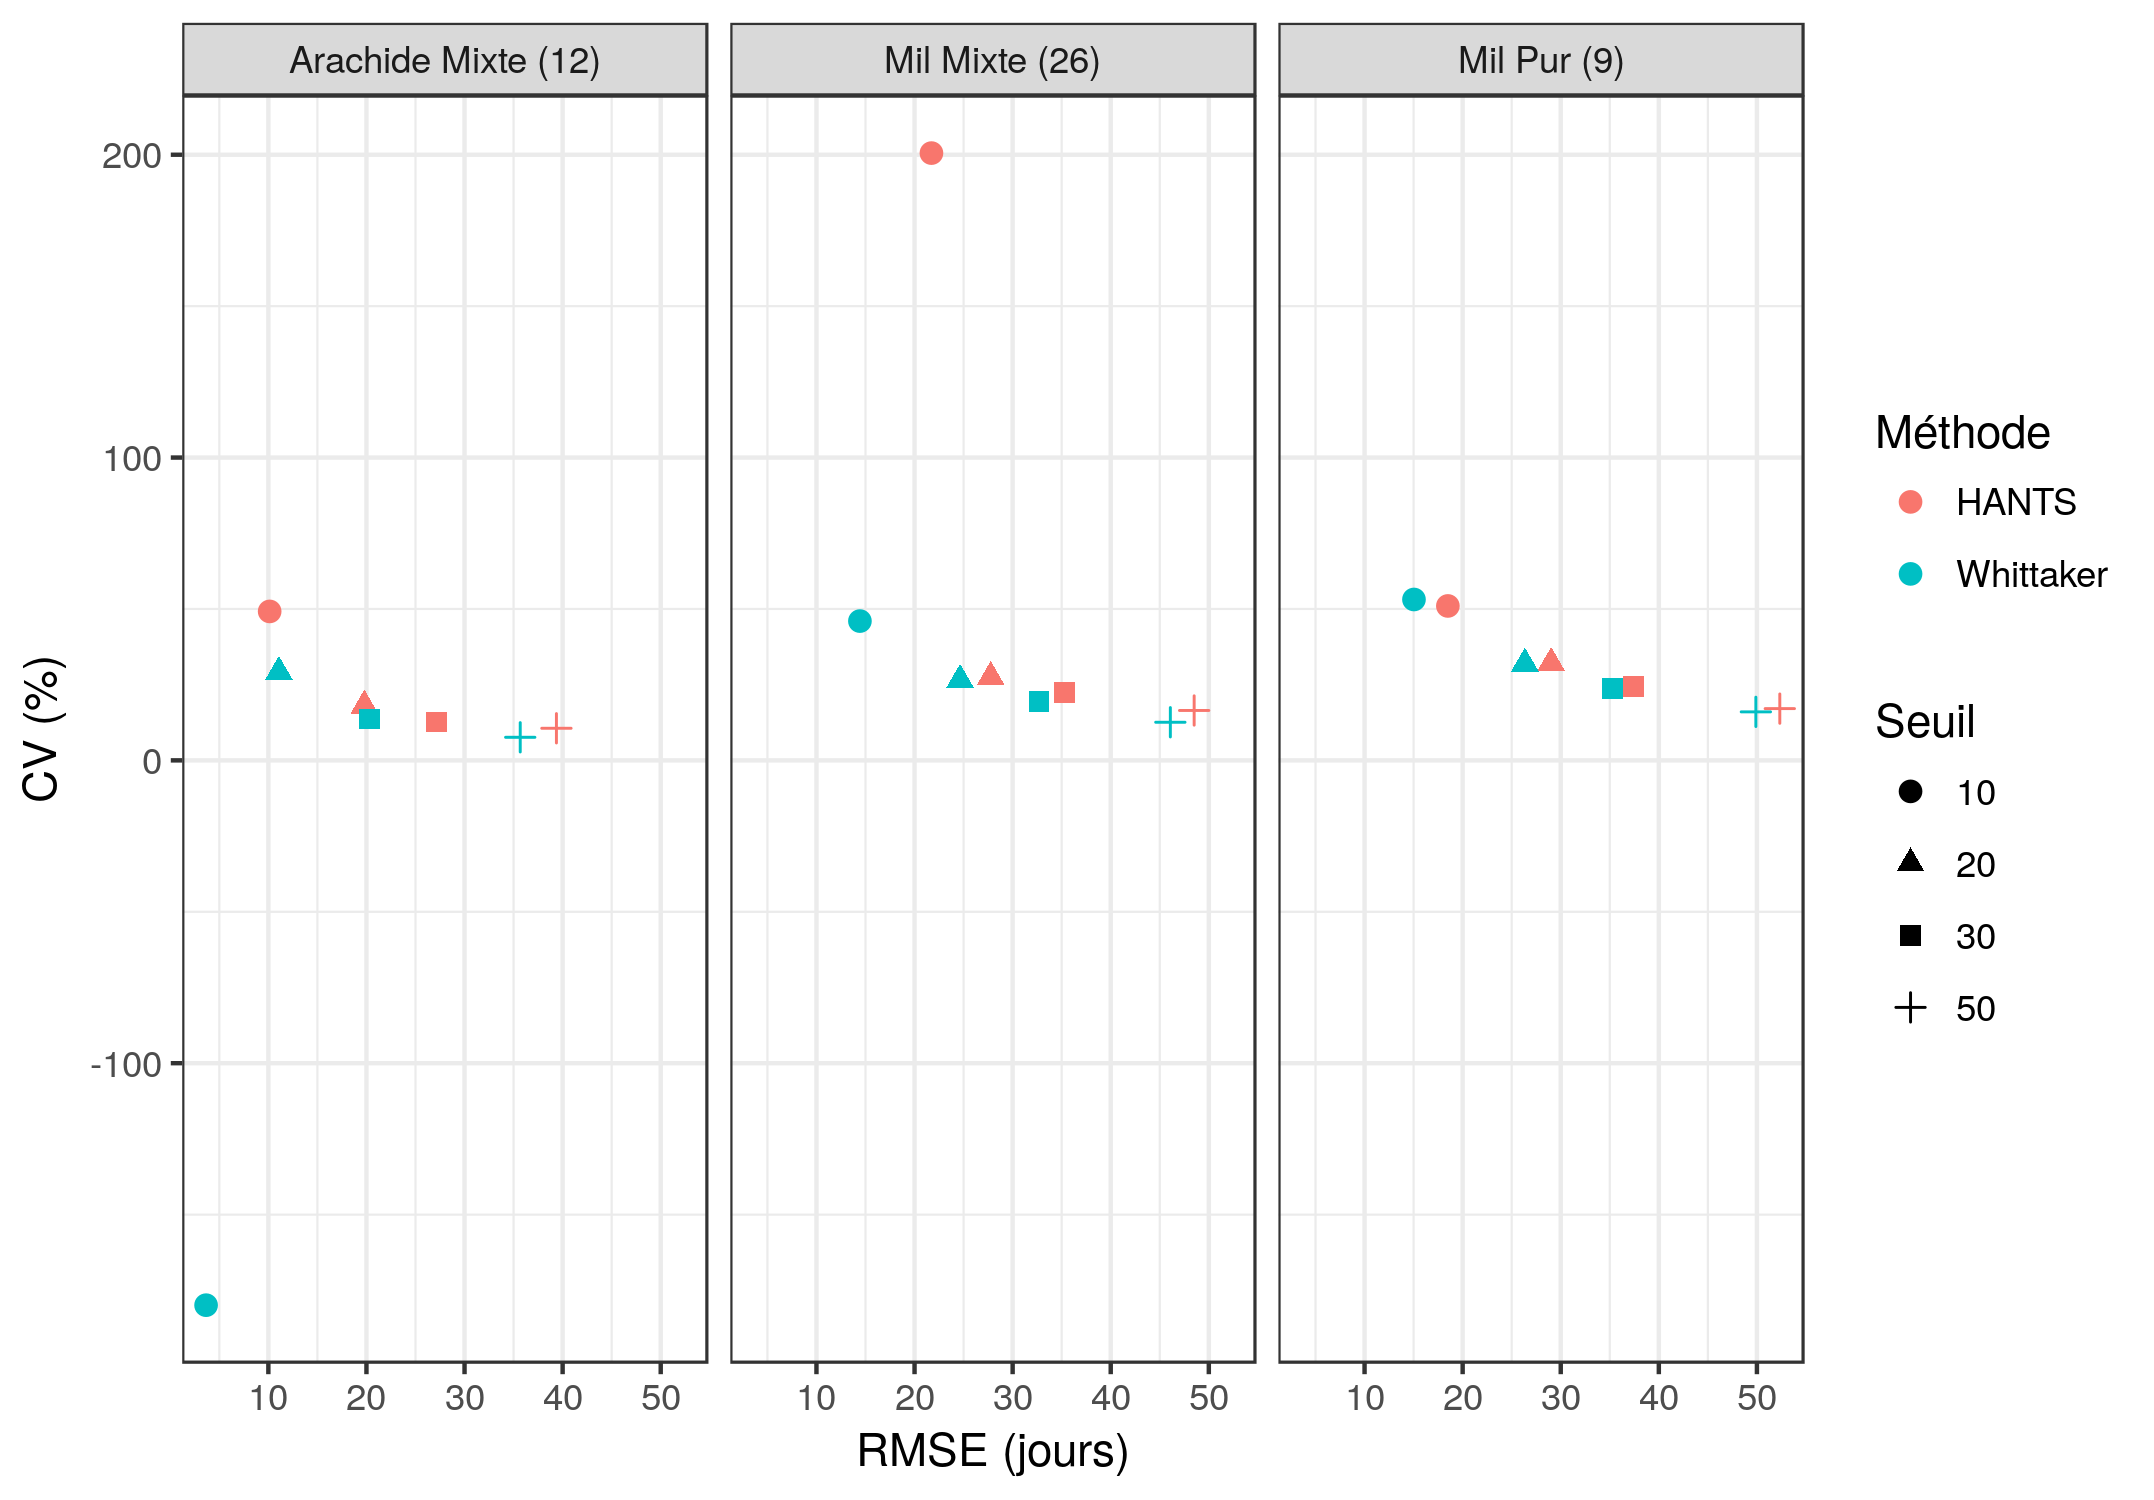
\includegraphics[scale=0.7]{resultats_discussions/SOS_RMSE_vs_CV.png} 
 \end{center}
 \caption[SOS -- RMSE vs CV]{Représentation du RMSE entre dates de semis et SOS estimés en fonction du coefficient de variation de leurs écarts par système de culture et méthode de lissage}
 \label{fig-sos-rmse-cv}
\end{figure}

\begin{figure}[htbp]
 \begin{center}
  \includegraphics[scale=0.7]{resultats_discussions/Spatial_SOS.png} 
 \end{center}
 \caption[Spatialisation des SOS]{Spatialisation des SOS extraits à l'échelle pixellaire (3 mètres) sur la zone d'application du lissage}
 \label{fig-spatial-sos}
\end{figure}

\paragraph{EOS}
Comme pour les SOS, nous avons représenté la distribution des écarts mais cette fois ci entre les dates de récoltes observées et les EOS extraits par système de culture et méthode de lissage (\Cref{fig-eosboxplot}). Les parcelles d'arachide mixte montrent légèrement moins de variabilité entre les écarts que les parcelles de mil mixte et de mil pur. La plage des écarts obtenus avec les EOS estimés par HANTS semble légèrement inférieure à celle des écarts obtenus avec les EOS extraits par la méthode de Whittaker notamment pour tous les seuils sur les parcelles d'arachide mixte. Néanmoins, les écarts obtenus avec HANTS sont nettement inférieurs à ceux de la méthode de Whittaker quand on considère le même seuil et tous les sytèmes de culture confondus. En ce qui concerne la variation des seuils, plus ils sont grands et plus les dates de fin de saison estimées se rapprochent 
des dates de récoltes que ce soit pour les parcelles d'archide ou de mil. Néanmoins, le seuil de 60\% extrait des EOS précoces pour les parcelles d'arachide mixte (médiane des écarts autour de $0$ pour les 2 méthodes de lissage) tandis que les EOS extraits pour les parcelles de mil avec un seuil de 80\% ont au moins 10 jours d'écart avec les dates de récoltes. Le seuil le plus adapté pour chaque système de culture doit déterminer les EOS en minimisant la variabilité des écarts par rapport aux dates de récoltes et en les minimisant au mieux puisqu'en fin de compte les périodes de forte corrélation pour l'estimation des rendements qui viendra par la suite, ne devraient pas excéder les dates de récoltes. Référons nous alors à la \cref{fig-eos-rmse-cv}. Pour les parcelles d'arachide mixte, les RMSE les plus faibles sont obtenus avec les seuils de 60 et 70\% ce qui est normal car les écarts entre EOS et dates de récoltes à ces seuils sont faibles. Par contre, leurs coefficients de variations très élevés rappellent le cas de dates précoces comme pour le SOS. 

\begin{figure}[htbp]
 \begin{center}
  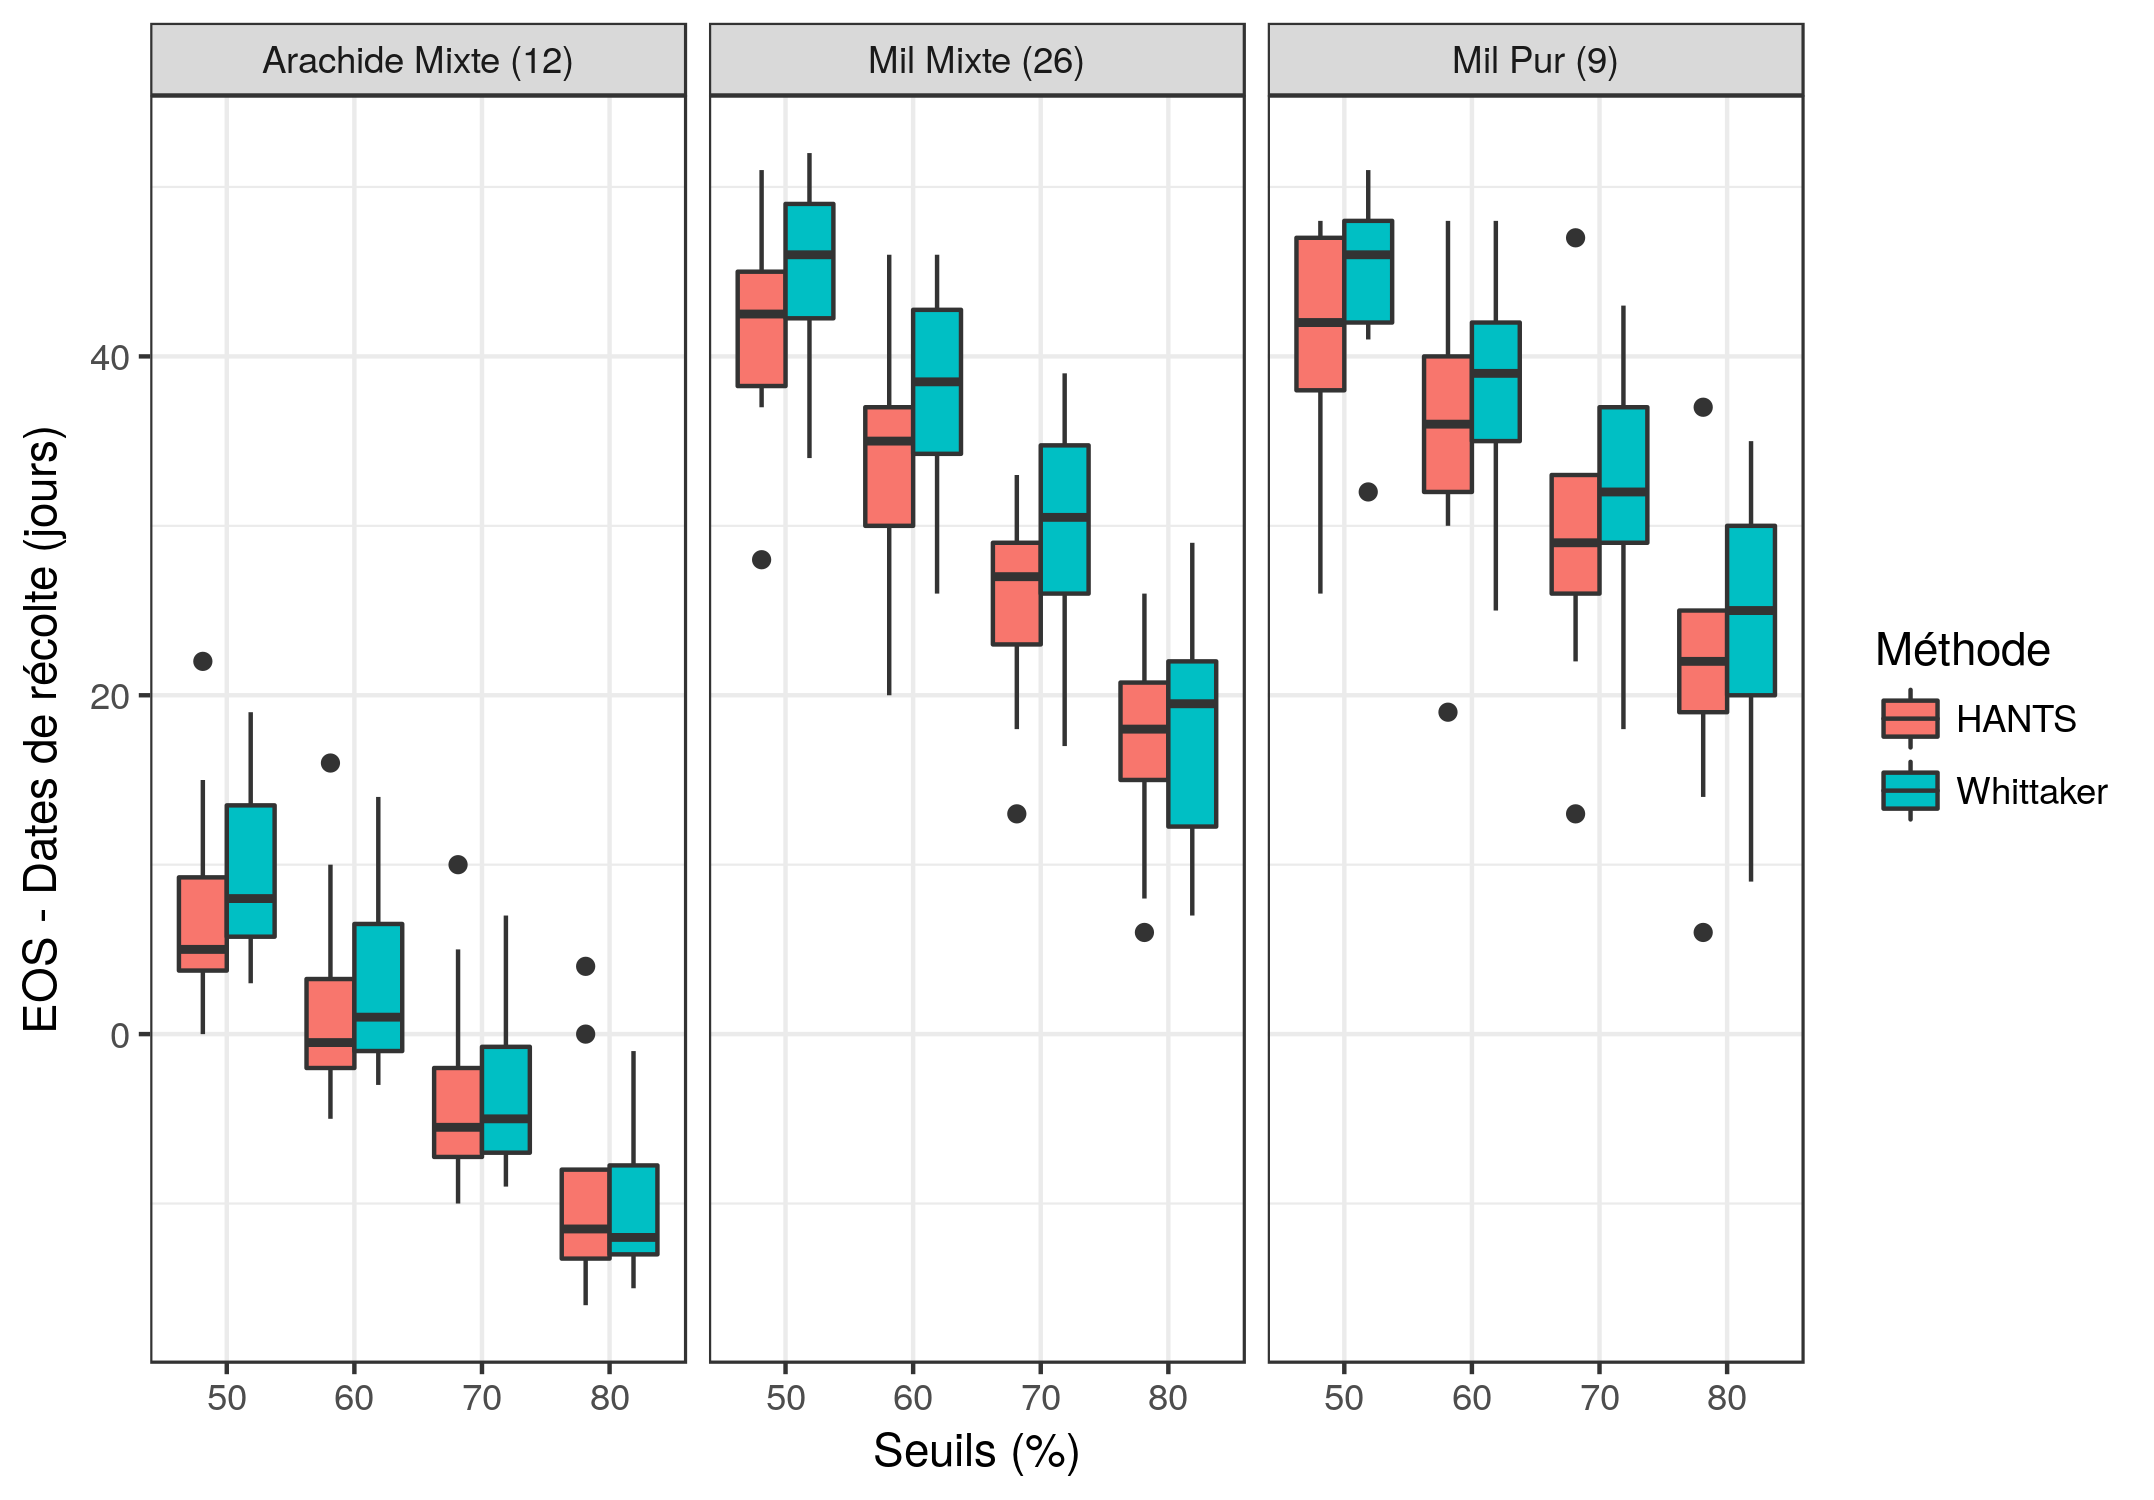
\includegraphics[scale=0.7]{resultats_discussions/EOS_Boxplot.png} 
 \end{center}
 \caption[Distribution des écarts entre EOS et dates de récoltes]{Boîtes à moustaches illustrant la distribution des écarts entre EOS estimés et dates de récoltes observées en fonction des systèmes de culture et des méthodes de lissage}
 \label{fig-eosboxplot}
\end{figure}

\begin{figure}[htbp]
 \begin{center}
  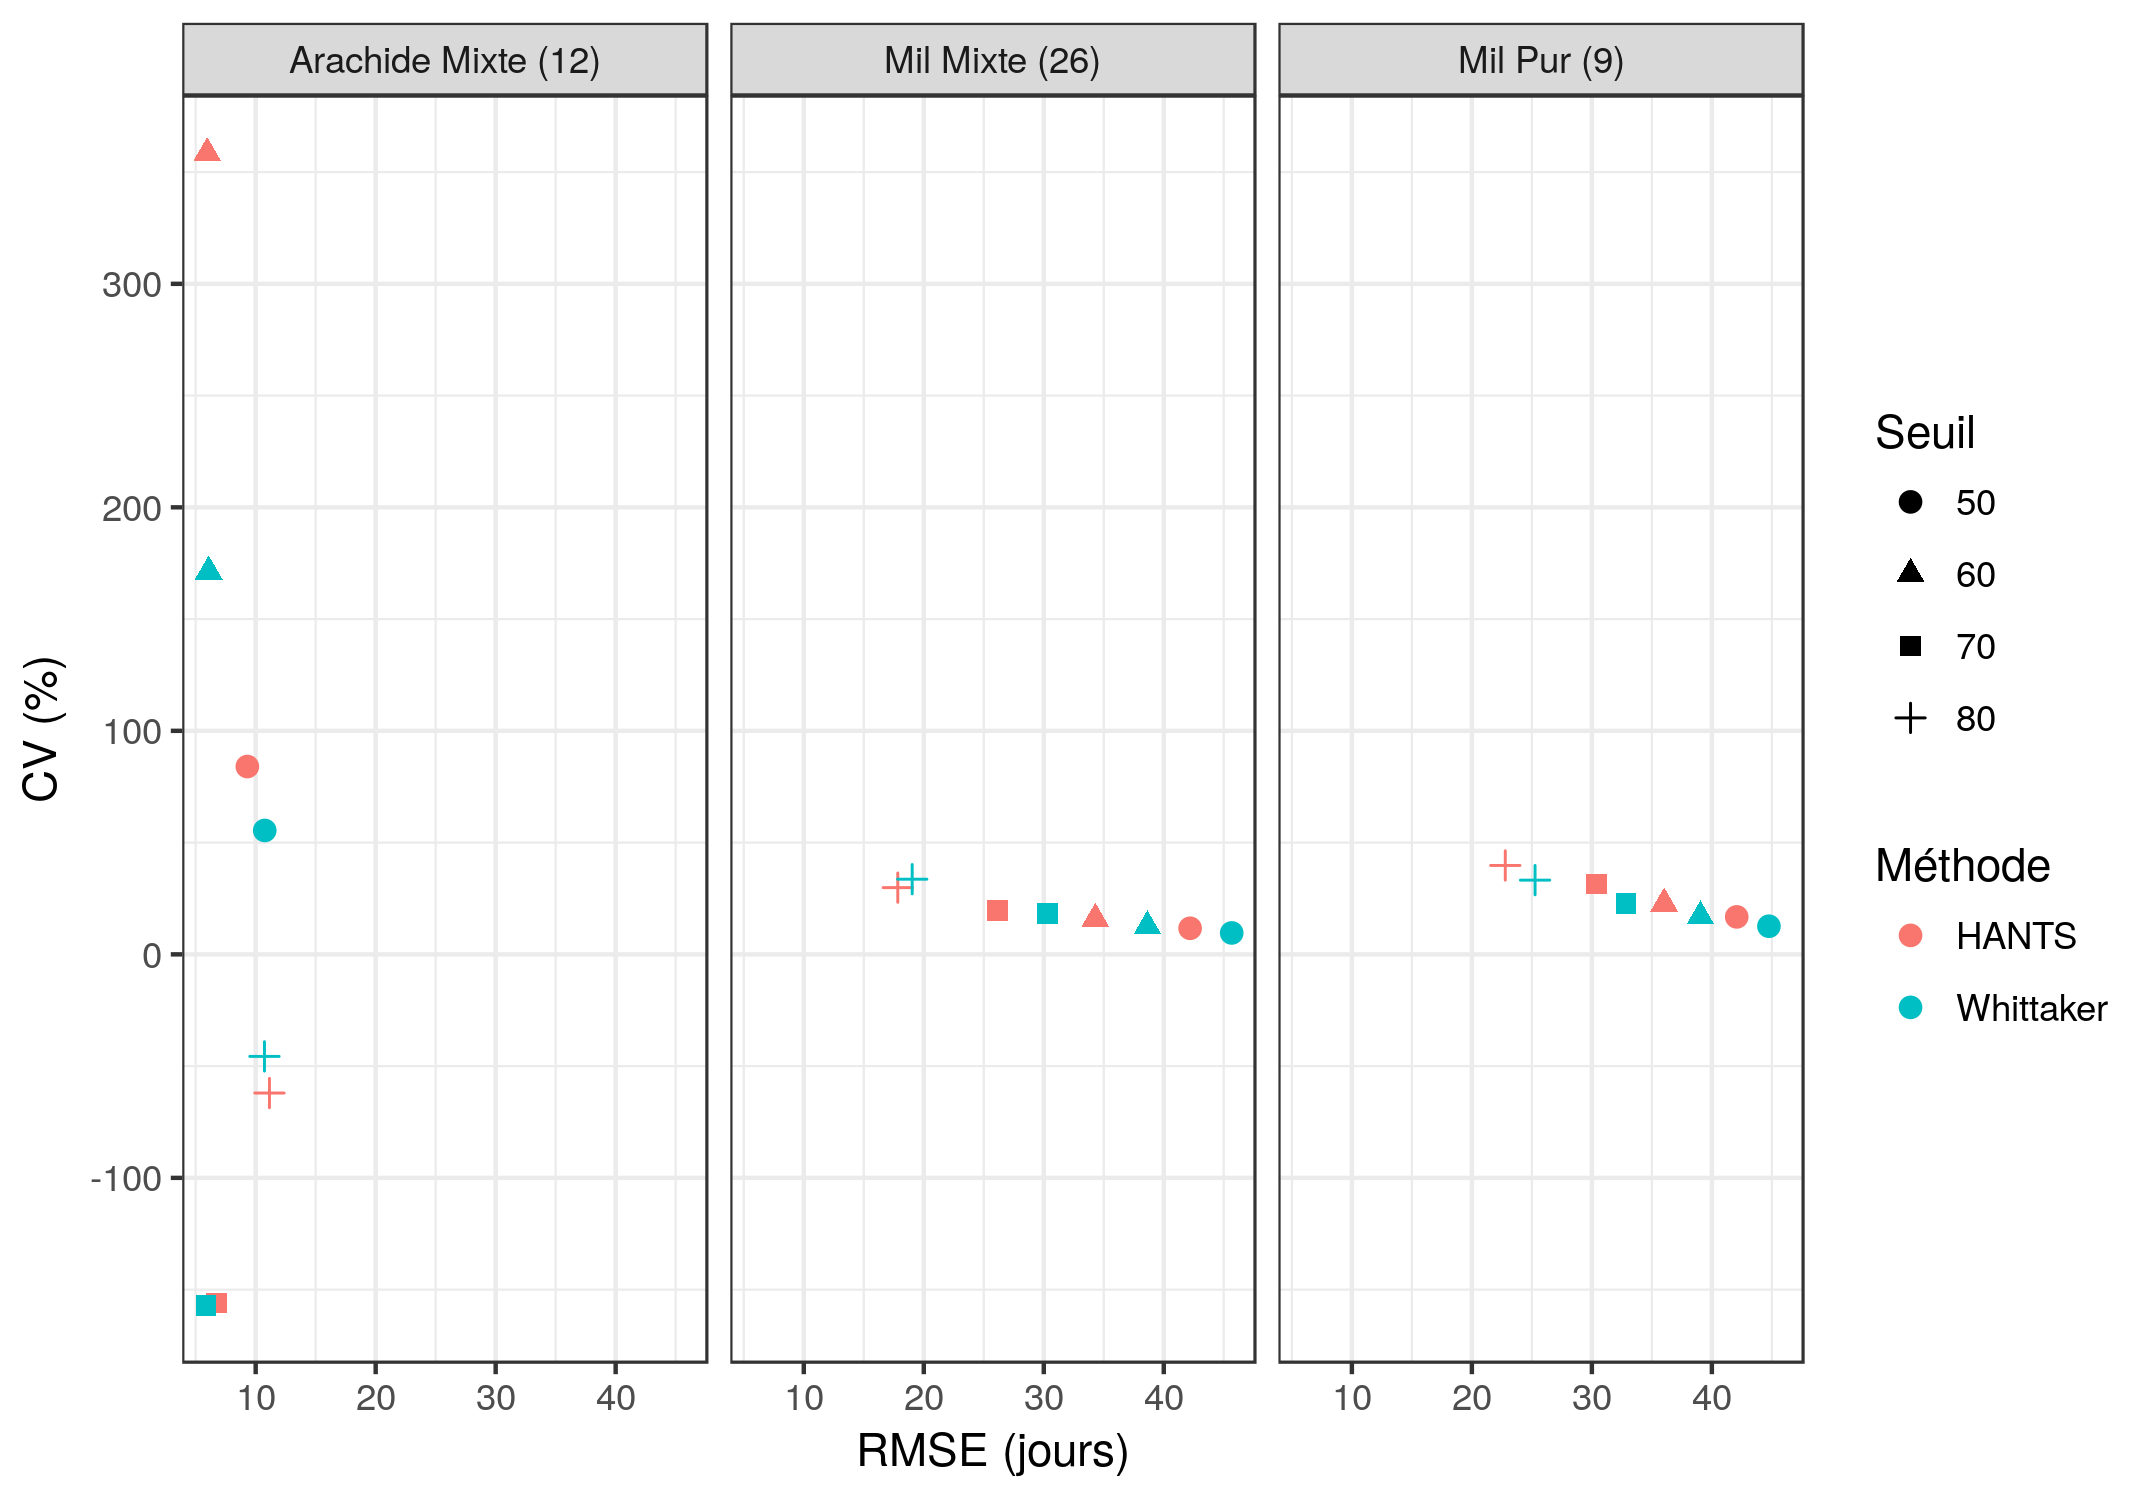
\includegraphics[scale=0.7]{resultats_discussions/EOS_RMSE_vs_CV.png} 
 \end{center}
 \caption[EOS -- RMSE vs CV]{Représentation du RMSE entre EOS estimés et dates de récoltes observées en fonction du coefficient de variation de leurs écarts par système de culture et méthode de lissage}
 \label{fig-sos-rmse-cv}
\end{figure}


\subsection{Estimation des rendements}
  
\section{Discussions}

\subsection{Sur l'extraction du SOS et du EOS}

\subsection{Sur l'estimation des rendements}

  
  \chapter{Conclusion et Perspectives}
  
  Ce travail a été réalisé dans le contexte de l’évaluation spatialisée par télédétection
des systèmes de cultures à base de mil et d’arachide dans le bassin arachidier du
Sénégal. Dans cette perspective, il avait pour objectif principal d’évaluer le potentiel
d’une série temporelle multisource (Sentinel-2, RapidEye et PlanetScope) à travers
deux sous objectifs : l’évaluation des dates de semis et l’estimation des biomasses vé-
gétatives et des rendements grains du mil et gousses de l’arachide.
\\En lissant les profils temporels de NDVI extraits à partir de la série multisource,
notamment avec la méthode de Whittaker, nous avons extrait différentes métriques
phénologiques dont les dates de début de croissance de la végétation (SOS). Avec les
SOS extraits, nous avons estimé les dates de semis des différents systèmes de culture
avec notamment plus ou moins 5 jours de décalage pour les parcelles d’arachide et
10 à 20 jours de décalage pour celles de mil. Pour l’estimation des biomasses et ren-
dements, le NDVI, qui est traditionnellement utilisé, a été comparé à un autre indica-
teur de productivité de la végétation, le GDVI. Nous avons montré que le NDVI était
moins performant que le GDVI pour expliquer la variabilité de la biomasse et des
rendements, ceci s’expliquant notamment par un changement dans les technologies
d’observation de la Terre par rapport aux études précédentes. Cette étude a montré
le réel intérêt de combiner différentes sources d’images satellitaires afin d’améliorer
la répétitivité de l’information spatiale. Elle a également montré que la différence de
résolutions spatiales entre les types d’images ne représente en aucun cas un frein à
leur utilisation combinée au sein d’une même application.
\\Néanmoins, au vu des résultats obtenus, la méthodologie mise en place pourrait être
affinée, notamment pour améliorer la partie estimation des biomasses et rendements.
Dans un ordre de priorité, notre première recommandation concerne la phase de
prétraitements des images qui pourrait inclure des corrections atmosphériques afin
d’uniformiser tout le jeu données. En effet, seules les images Sentinel-2A dans notre
série temporelle multisource présentaient des corrections atmosphériques et nom-
breuses sont les études en télédétection ayant fait état du gain significatif que ces
corrections pouvaient apporter. Dans notre série temporelle, nous n’avons utilisé que
les images Sentinel-2A. Sentinel-2B étant aujourd’hui opérationnel, un couplage des
2 types d’images viendrait densifier notre série temporelle afin d’éviter des périodes
sans informations comme cela a été le cas pendant le mois de Septembre dans notre
étude. Également sur ce point, l’utilisation d’images radar pourrait être une solution
envisageable quand on sait que le principal avantage de l’imagerie radar se trouve
dans l’affranchissement des conditions atmosphériques, nuages notamment. L’adop-
tion d’images radars permettrait également de tester un apport éventuel des indices
radar pour l’extraction des SOS et EOS et l’estimation des biomasses et rendements.
En ce qui concerne les méthodes de lissage, s’il est vrai qu’elles ont plutôt donné
satisfaction, il n’en est pas moins que cette étape influence fortement les résultats
obtenus par la suite. Il serait alors intéressant de tester d’autres types d’approches
comme les fonctions asymétriques gaussiennes ou les doubles fonctions logistiques dont les résultats sont jugés tout autant satisfaisants. Aussi, la grande majorité de
notre travail a été basé sur l’utilisation du NDVI qui a montré ses limites pour l’es-
timation des biomasses et rendements. Dès lors, il serait pertinent de se tourner vers
d’autres indices de végétation comme cela a déjà pu être le cas avec le GDVI. D’autres
indicateurs comme le MSAVI qui tient compte de l’effet des sols (intéressant dans
le cas de cultures peu couvrantes comme le mil), le NDWI pouvant détecter la pré-
sence de stress hydrique chez les cultures ou encore les indices explorant la bande
du red edge comme le Red Edge NDVI pourraient être de réelles alternatives. Par
ailleurs, l’extraction des métriques phénologiques a été réalisée uniquement à partir
de la méthode de seuillage relatif sur les amplitudes de NDVI et il serait intéressant
de tester d’autres méthodes notamment les méthodes dérivatives. Outre cette étape,
celle de l’estimation des biomasses et rendements a tenu compte de variables expli-
catives provenant des seuls indices que sont le NDVI et le GDVI. Nous n’avons ni
exploré les variables biophysiques comme le LAI ni les variables climatiques comme
l’humidité du sol et les quantités de précipitations bien connues pour améliorer les
modèles calibrés. Les indices texturaux pourraient être également interessant à tester.
L’autre phase inexplorée également dans notre travail concerne la non prise en compte
du pouvoir explicatif des arbres (présents dans les parcelles) dans la productivité des
systèmes de cultures. Une des limites de notre travail aura été l’étroitresse de la taille
de notre jeu de données terrain rendant impossible la calibration de modèles multi-
variés plus robustes et leur validation. En effet, une taille d’échantillons plus grande
aurait permis l’implication de plusieurs variables dans nos modèles et aurait certaine-
ment amélioré les estimations de biomasses et rendements. D’autre part, augmenter
la taille de nos échantillons permettrait d’envisager le recours à des méthodes de ré-
gression plus poussées par fouilles de données telle que les forêts aléatoires d’arbres
décisionnels pour l’estimation des biomasses et rendements. Une autre limite de notre
travail repose sur la qualité des données de biomasses et de rendements observés. Ef-
fectivement, ces données ayant été collectées dans la cadre d’autres projets et donc
pas initialement pour l’estimation des biomasses et rendements, il nous aura été im-
possible de savoir jusqu’à quel point nous y fier. Sur ce point, un nouveau réseau de
parcelles est en cours de suivi pour la campagne agricole 2018. Ce nouveau jeu de
données sera ajouté à celui de la campagne 2017 sur laquelle nous avons travaillé et
viendra élargir la taille d’échantillons pour les estimations de biomasses et de rende-
ments de 2018. Pour finir, une évaluation spatialisée des rendements dans la région
du bassin arachidier sénégalais requiera avant tout un masque des principaux sys-
tèmes de cultures présents. Ce type de données est obtenu par classification. Dans le
cadre du projet S2-Agri\footnote{\url{http://www.esa-sen2agri.org/}} , un outil a été mis en place pour la production de masques
de cultures ainsi que des cartes d’occupation du sol spécialisées sur l’agriculture.

  
\appendix

\chapter{Diagramme de Gantt}\label{annexe-a}

\backmatter
\newacronym{cirad}{Cirad}{Centre de Coopération Internationale pour la Recherche Agronomique et le Développement} 
\newacronym{aida}{UR Aïda}{Unité de Recherche Agroécologie et intensification durable des cultures annuelles, Cirad}
\newacronym{isra}{ISRA}{Institut Sénégalais de Recherche Agronomique}
\newacronym{cse}{CSE}{Centre de Suivi Ecologique}
\newacronym{ndvi}{NDVI}{Normalized Difference Vegetation Index --- Indice de végétation par différence normalisé}
\newacronym{evi}{EVI}{Enhanced Vegetation Index}
\newacronym{lsp}{LSP}{Land Surface Phenology}
\newacronym{savi}{SAVI}{Soil Adjusted Vegetation Index}
\newacronym{msavi}{MSAVI}{Modified Soil Adjusted Vegetation Index}
\newacronym{sos}{SOS}{Start of Season --- Démarrage de croissance de la végétation}
\newacronym{eos}{EOS}{End of Season --- Fin de croissance de la végétation}
\newacronym{pos}{POS}{Peak of Season --- Maximum de croissance de la végétation}
\newacronym{gsl}{GSL}{Growing Season Length --- Durée de croissance de la végétation = EOS -- SOS}
\newacronym{toa}{TOA}{Top of Atmosphere --- Radiance ou Réflectance au sommet de l'atmosphère}
\newacronym{utm}{UTM}{Projection Transverse Universelle de Mercator; Zone 28N sur Niakhar}
\newacronym{mvc}{MVC}{Maximum Value Composite}
\newacronym{bise}{BISE}{Best Index Slope Extraction}
\newacronym{hants}{HANTS}{Harmonic Analysis of Time Series}
\newacronym{esa}{ESA}{European Spatial Agency --- Agence Spatiale Européenne}
\newacronym{gmes}{GMES}{Global Monitoring for Environment and Security}
\newacronym{envisat}{ENVISAT}{ENVIronment SATellite ---  Satellite d'observation de la Terre de l'ESA lancé en 2002 
dont l'objectif est de mesurer de manière continue à différentes échelles les principaux paramètres environnementaux de la Terre 
relatifs à l'atmosphère, l'océan, les terres émergées et les glaces}
\newacronym{msi}{MSI}{MultiSpectral Instrument}
\newacronym{theia}{Theia}{Pôle de données et de services surfaces continentales --- a pour objectif d’accroître l’utilisation par la 
communauté scientifique et les acteurs publics de la donnée spatiale en complémentarité d’autres types de données, notamment les 
données in situ et aéroportées}
\newacronym{muscate}{MUSCATE}{Atelier de production MUlti Satellite, multi-CApteurs, pour des données multi-TEmporelles mise en place par le CNES et le CESBIO au sein de Theia}
\newacronym{cnes}{CNES}{Centre National d'\'Etudes Spatiales français}
\newacronym{cesbio}{CESBIO}{Centre d'\'Etudes Spatiales de la BIOsphère}
\newacronym{maccs}{MACCS}{Multi-sensor Atmospheric Correction and Cloud Screening}
\newacronym{maja}{MAJA}{MACCS-ATCOR Joint Algorithm}
\newacronym{idr}{IDR}{Iterative interpolation for Data Reconstruction}

\printglossary[type=\acronymtype]

\cleardoublepage
\refstepcounter{chapter}
\addcontentsline{toc}{chapter}{\bibname}
\bibliographystyle{apalike}
\bibliography{bibliographie/serena}
  
\end{document}          
